\chapter{Produktion}

\section{Erstellung der Umgebung}

\subsection{Natur}

meer wurde mit animierten Texturen des ocean modifier gemacht
es wurden keine geometrie, sondern nur normals berechnet --> performance
diese wurde gebaket, und exportiert, und dann in den shader als normal map reingeladen
vier unterschiedliche texturen wurden reingeladen, zwei dawvon zweimal
alle wurden dann leicht unterschiedliche skaliert und rotiert, sodass ein tiling vermieden wird
--> sehr große herausforderung bei einer so großen oberfläche tiling zu vermieden
prozedurale textur da die textur animiert sein soll
außerdem wurden die wake-wellen des Bootes mit einer texture hinzugefügt
die textur-koordinaten dieser wellen, sind abhängig von einem Objekt, welches mit dem Boot mitgeführt wird
somit bewegen sich die wellen mit dem boot mit
als drittes feature hat die grundfläche mit dem wasser shader eine radiale gradient texture, sodass mit ausreichendem abstand von der kamera die Wasseroberfläche transparent wird, und somit sich dann zum Himmelüberblendet. Damit ist ein dunst effekt einfach zu faken.
grundsätzlich war das erstellen das hintergrundes eine herausforderung, da die filmaufnahmen zu unterschiedlichen zeitpunkten enstanden sind, und damit sich der himmel farblich und auch charakterlich (mal mehr mal weniger wolken) unterschieden hat. Somit wurde ein mittelweg mit sonnigem Hintergrund bei gleichzeitig möglichst vielen wolken entschieden
viele wolken heißt auch, dass sich im meer viel struktur spiegelt, was das bild realistischer erscheinen lässt

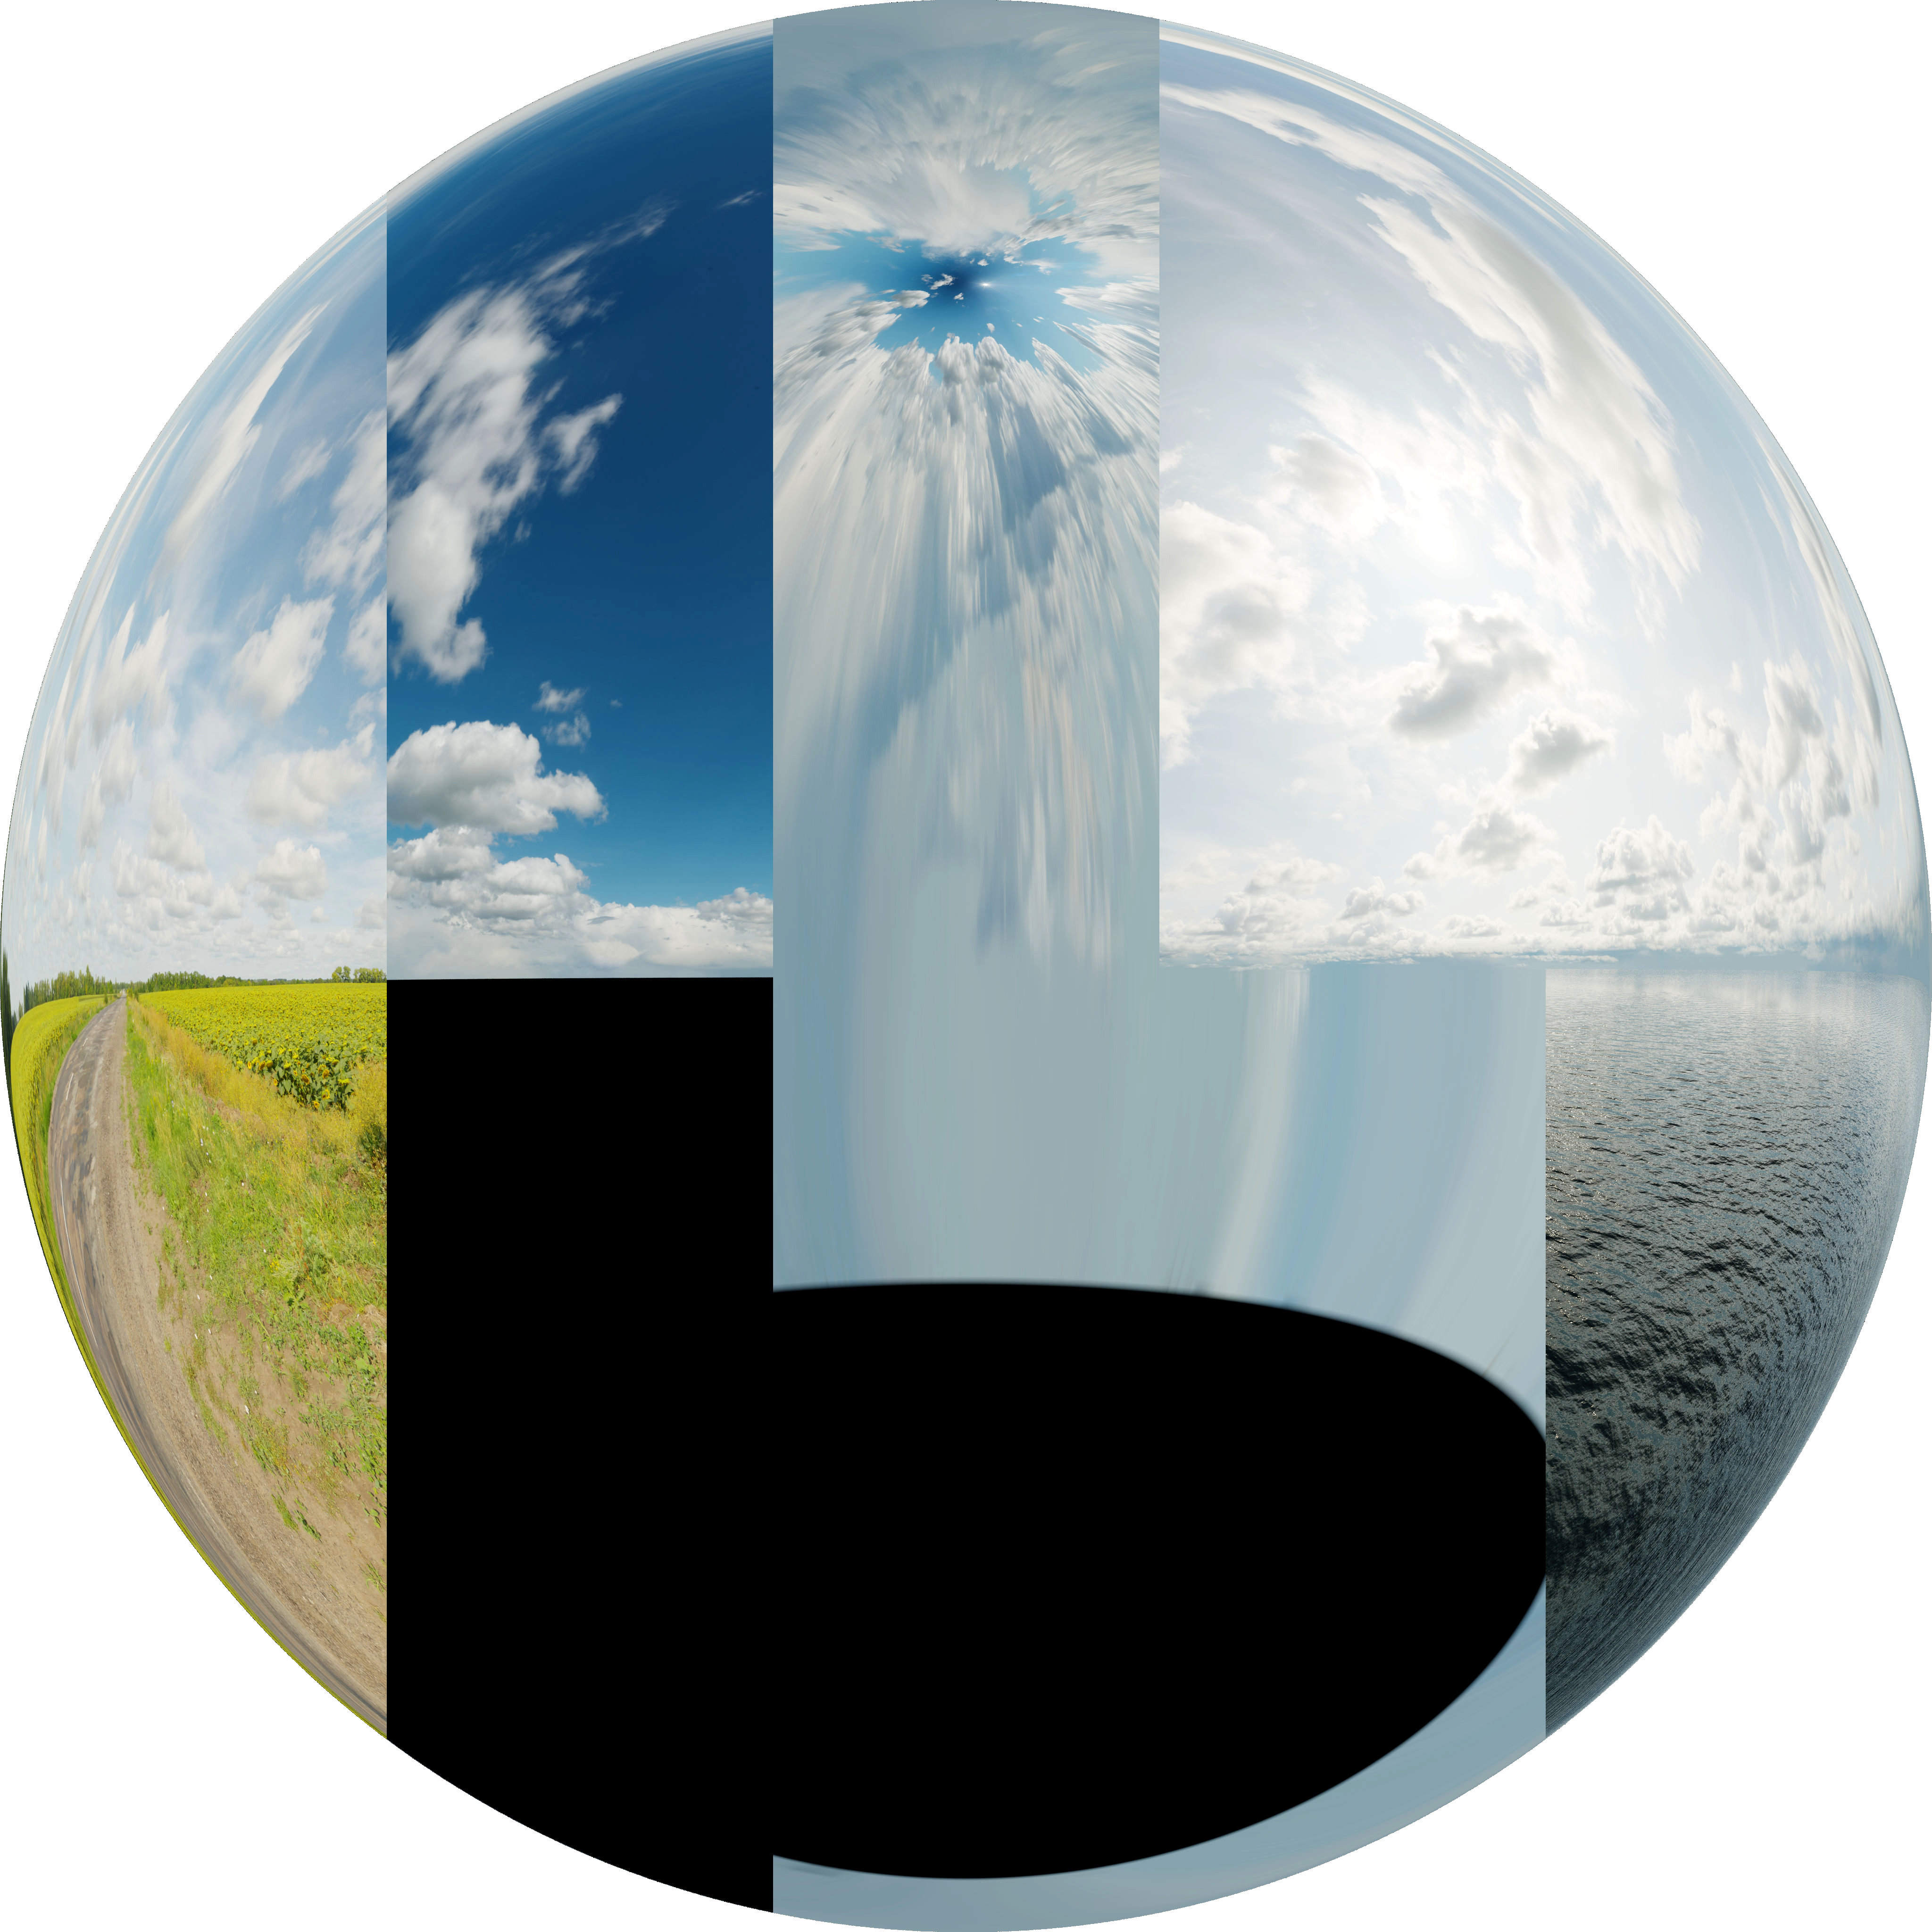
\includegraphics[width=\textwidth]{gfx/prod/env/env.jpg}
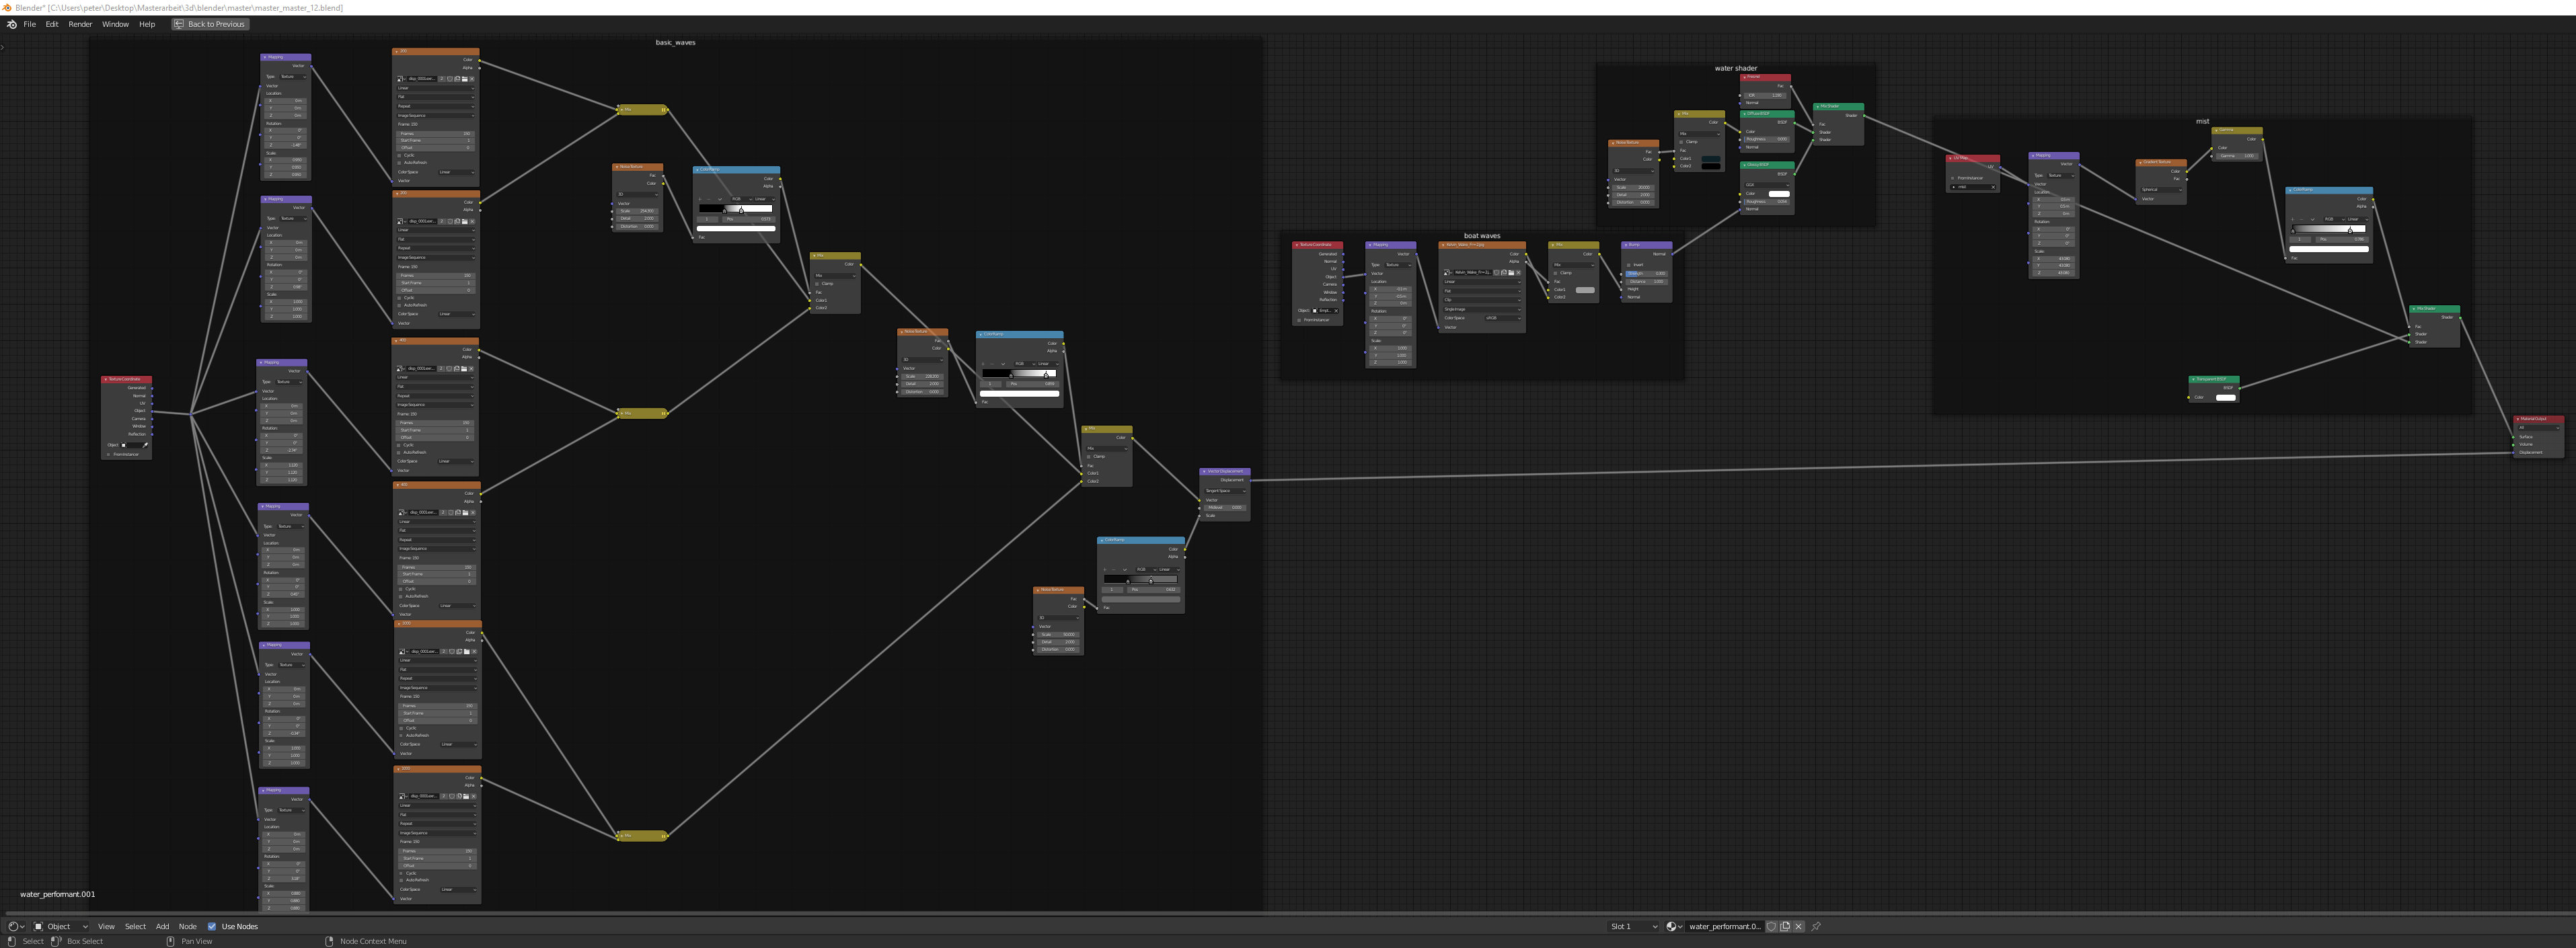
\includegraphics[width=\textwidth]{gfx/prod/env/ocean_shader.jpg}

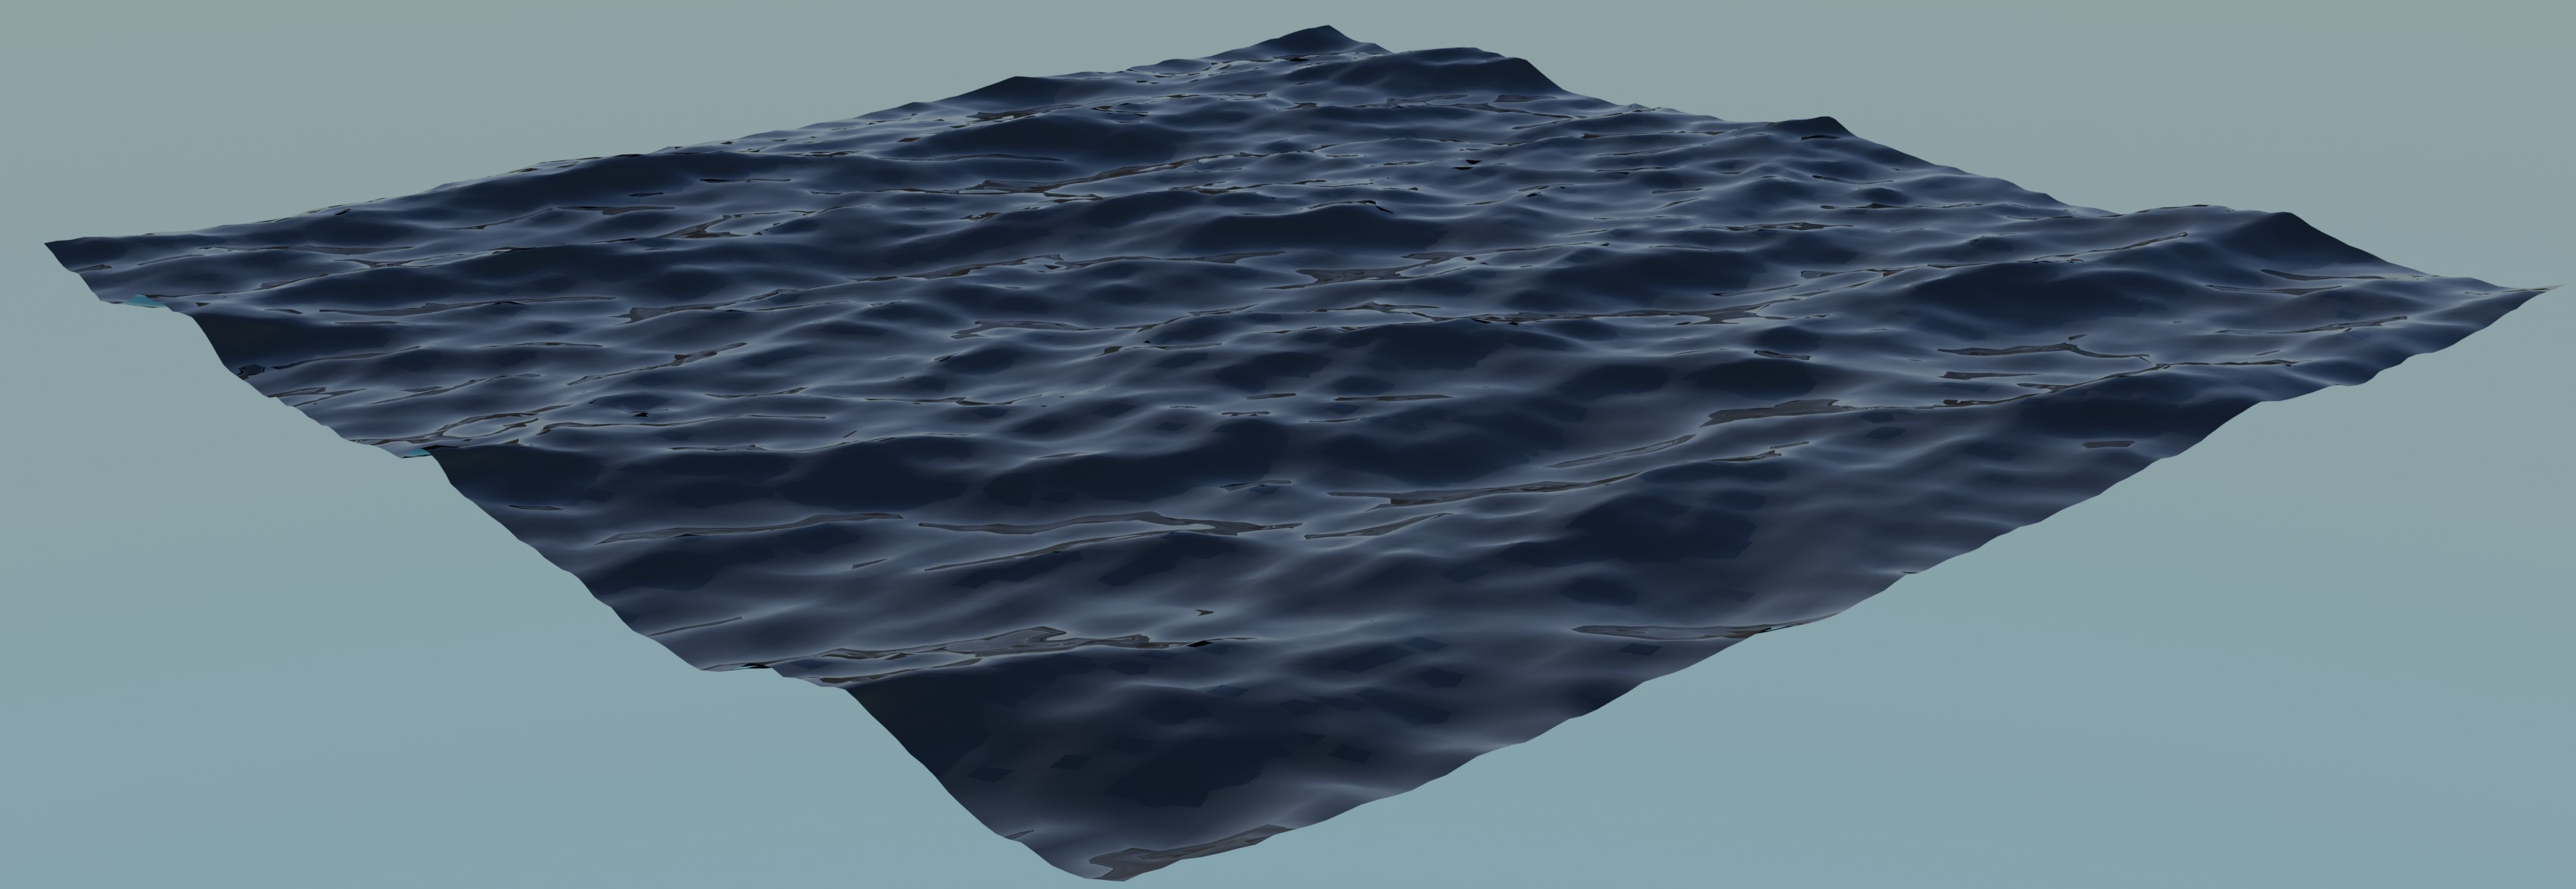
\includegraphics[width=\textwidth /2]{gfx/prod/ocean/meer0.jpg}
\includegraphics[width=\textwidth /2]{gfx/prod/ocean/meer1.jpg}
\includegraphics[width=\textwidth /2]{gfx/prod/ocean/meer2.jpg}
\includegraphics[width=\textwidth /2]{gfx/prod/ocean/meer3.jpg}
\includegraphics[width=\textwidth /2]{gfx/prod/ocean/meer4.jpg}
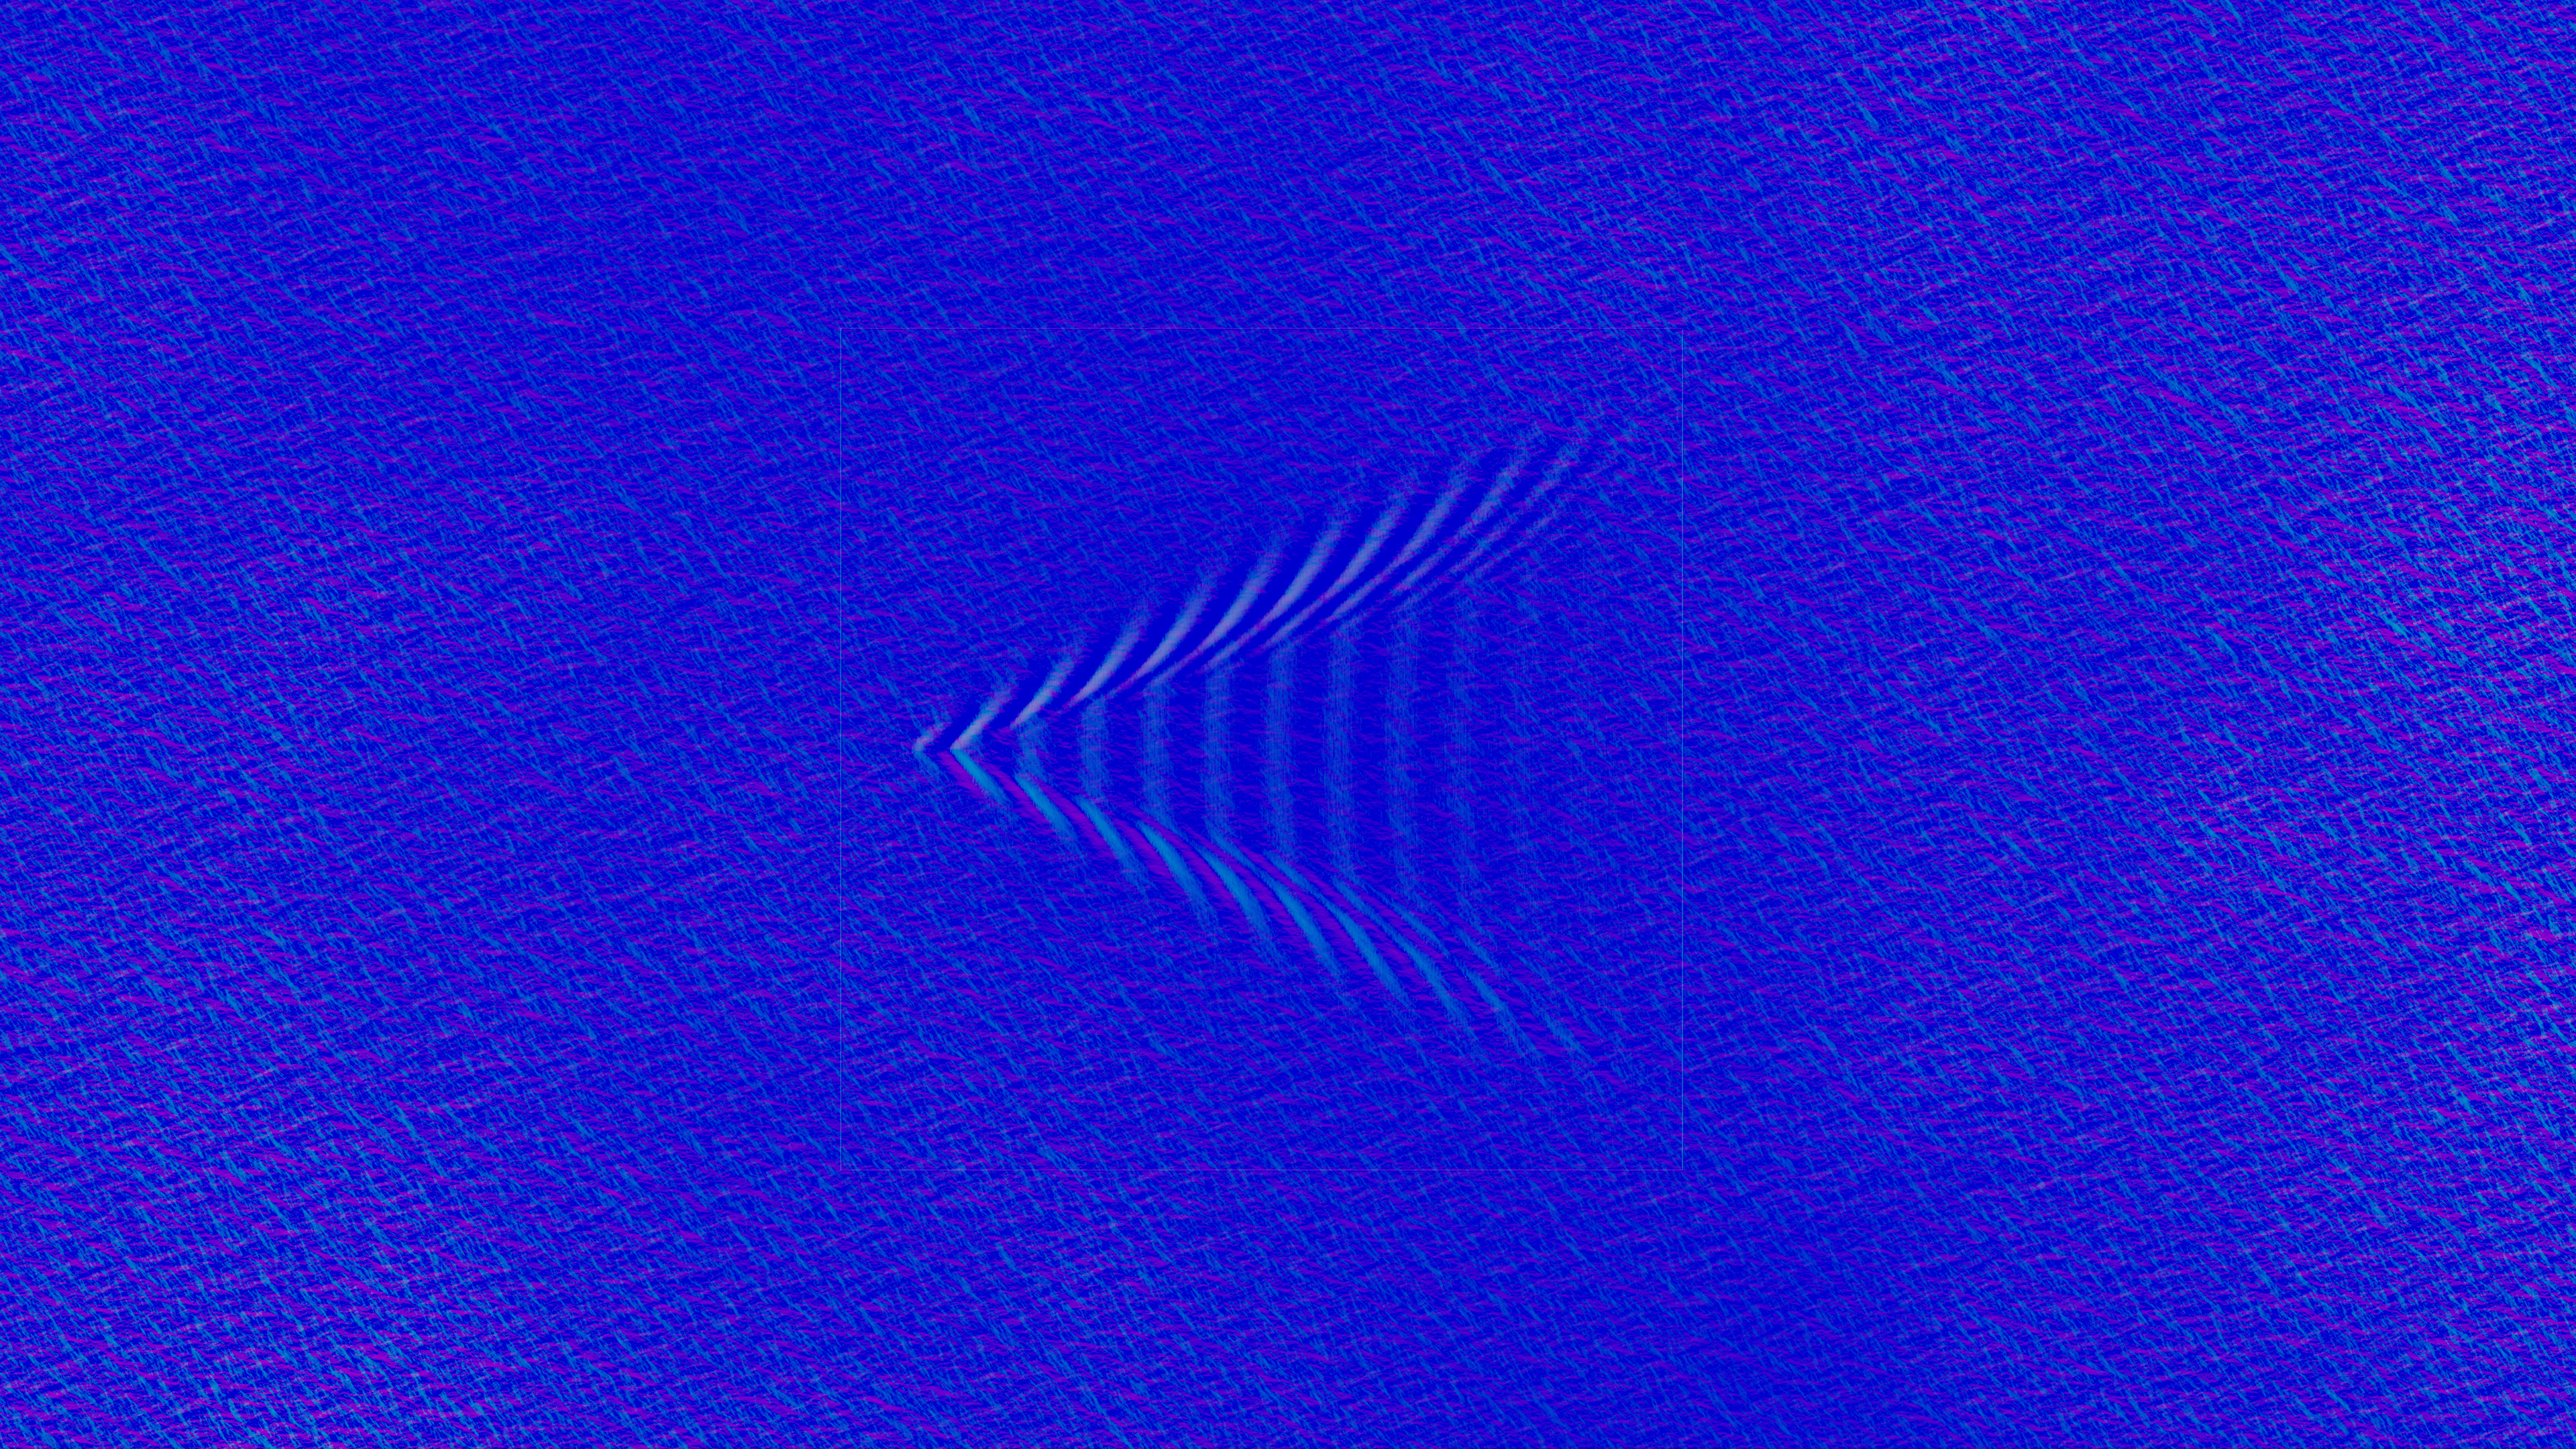
\includegraphics[width=\textwidth /2]{gfx/prod/ocean/meer5.jpg}
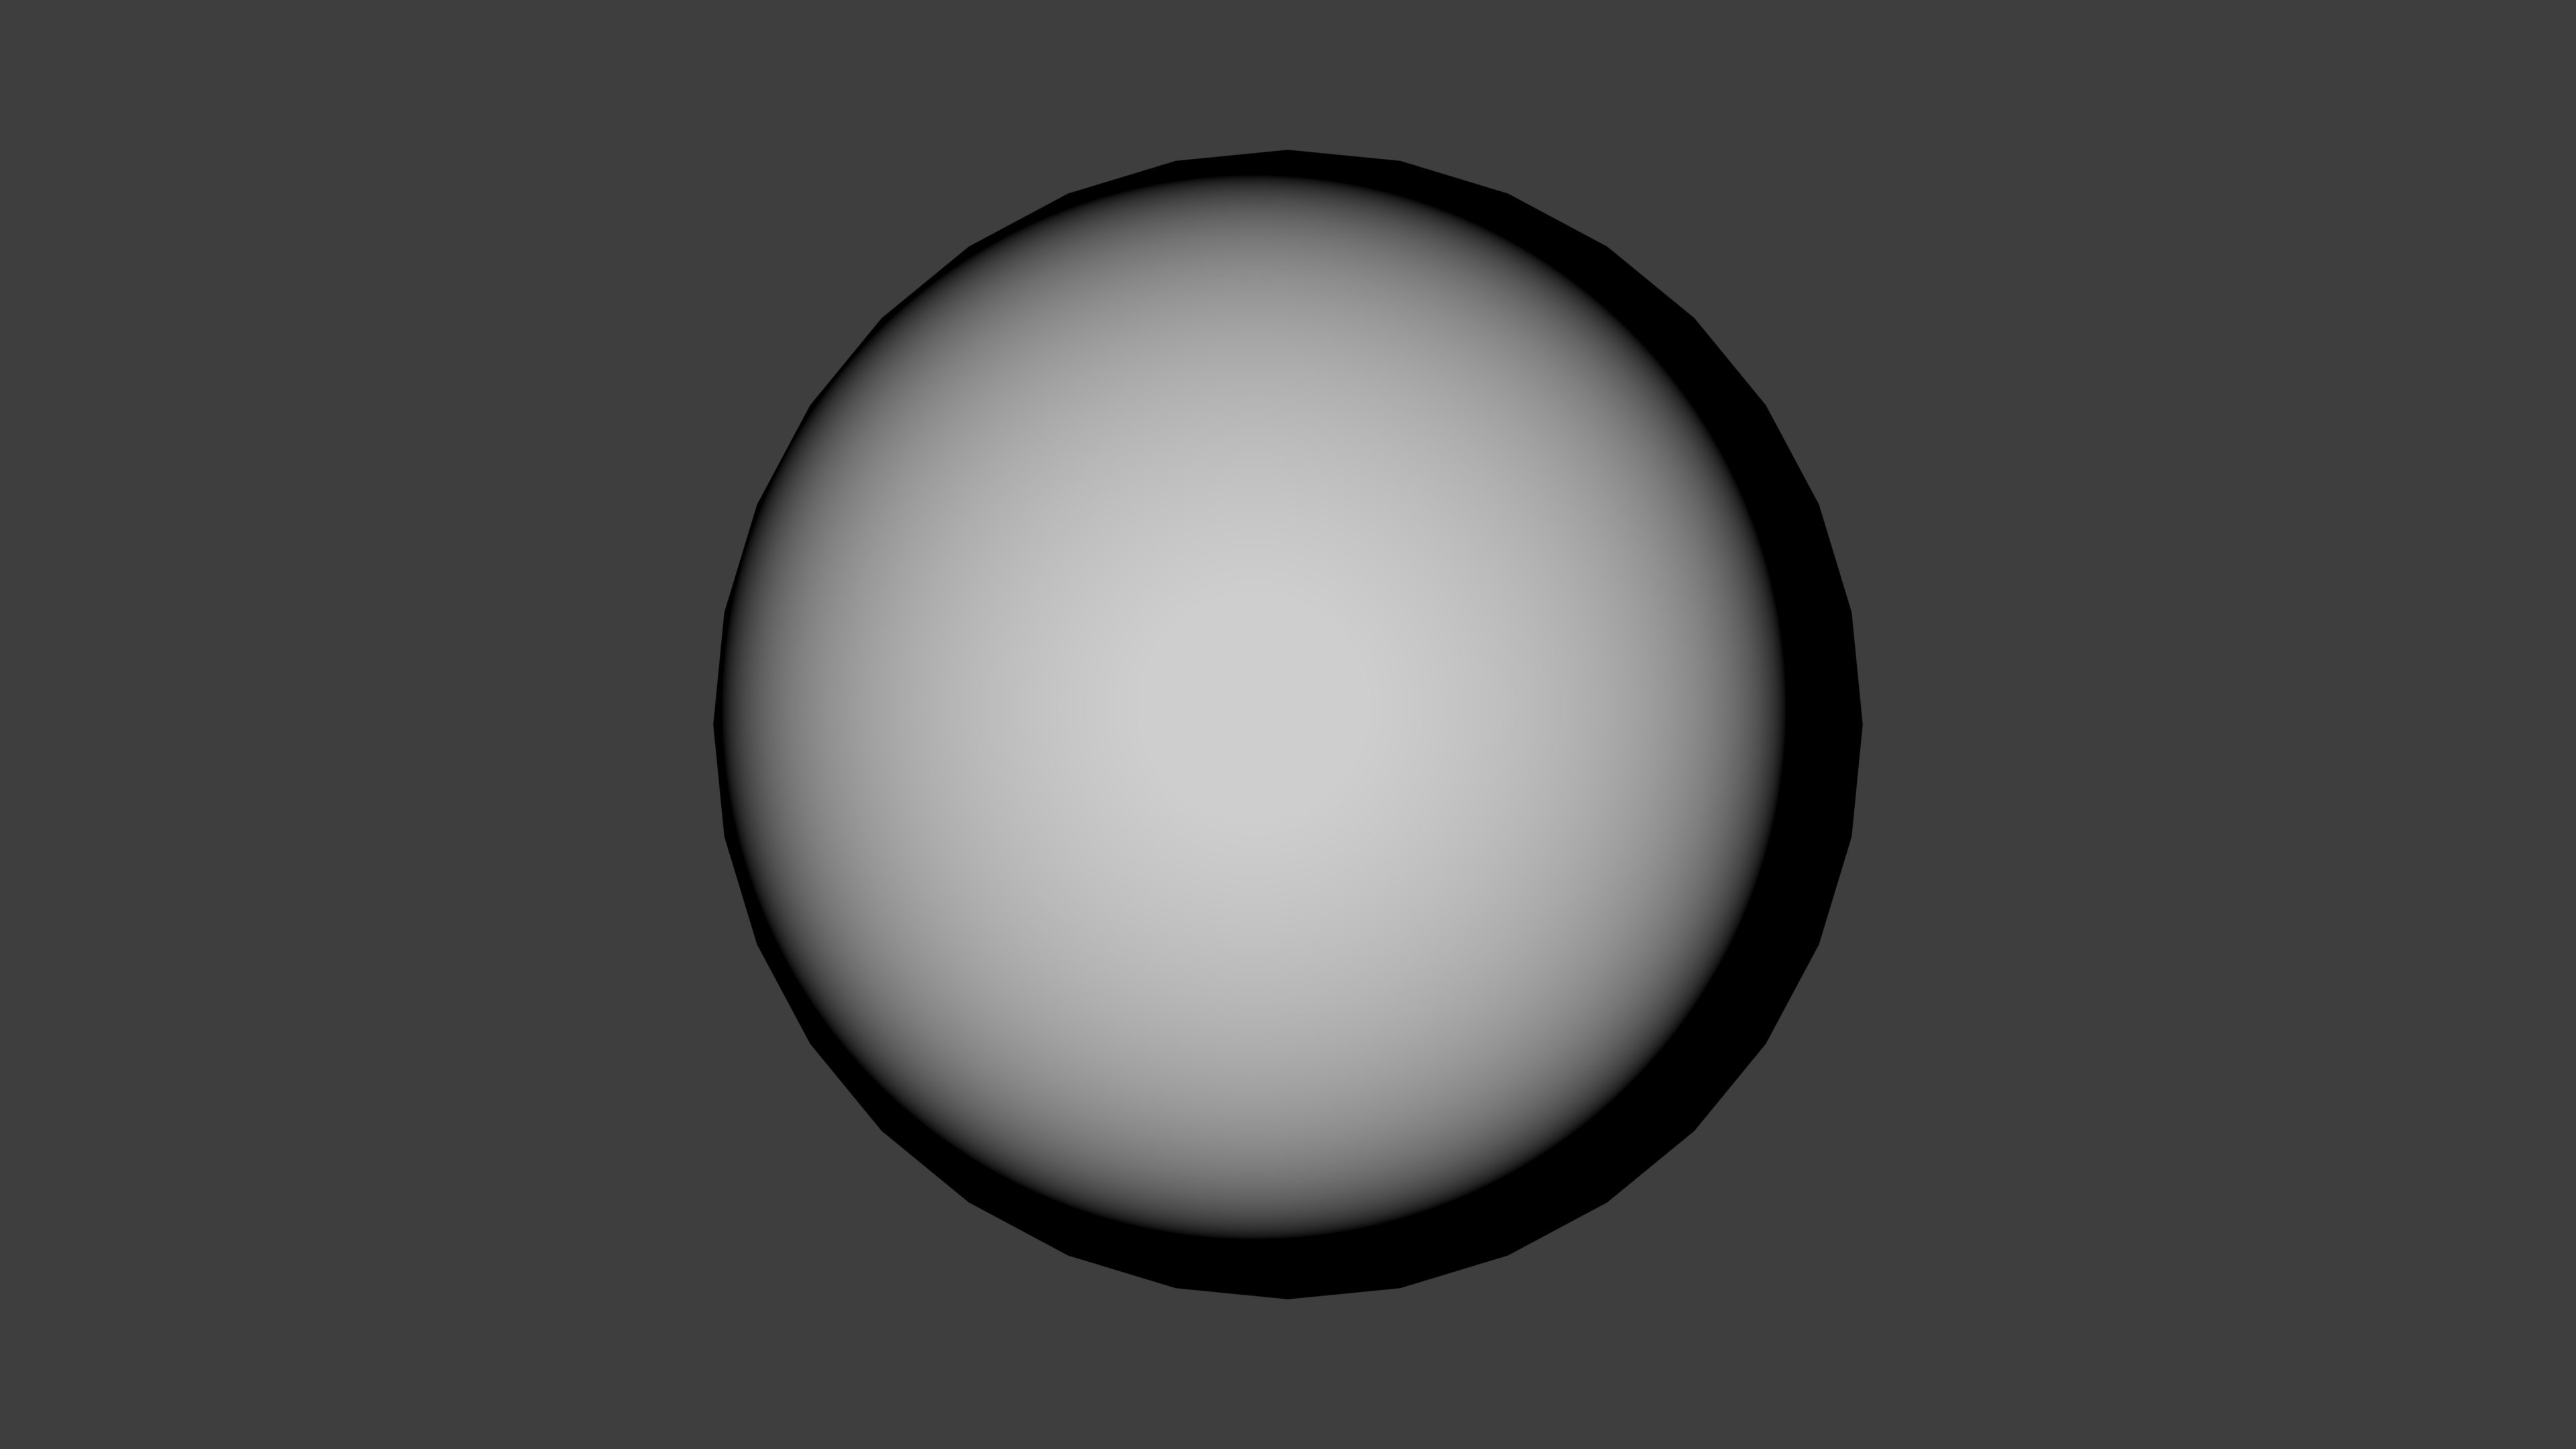
\includegraphics[width=\textwidth /2]{gfx/prod/ocean/meer6.jpg}

\includegraphics[width=\textwidth /2]{gfx/prod/ocean/meer7.jpg}


\subsection{Segelboot}

download von grabcad, import in blender im stl format
texturen und shader mussten noch eingefügt werden

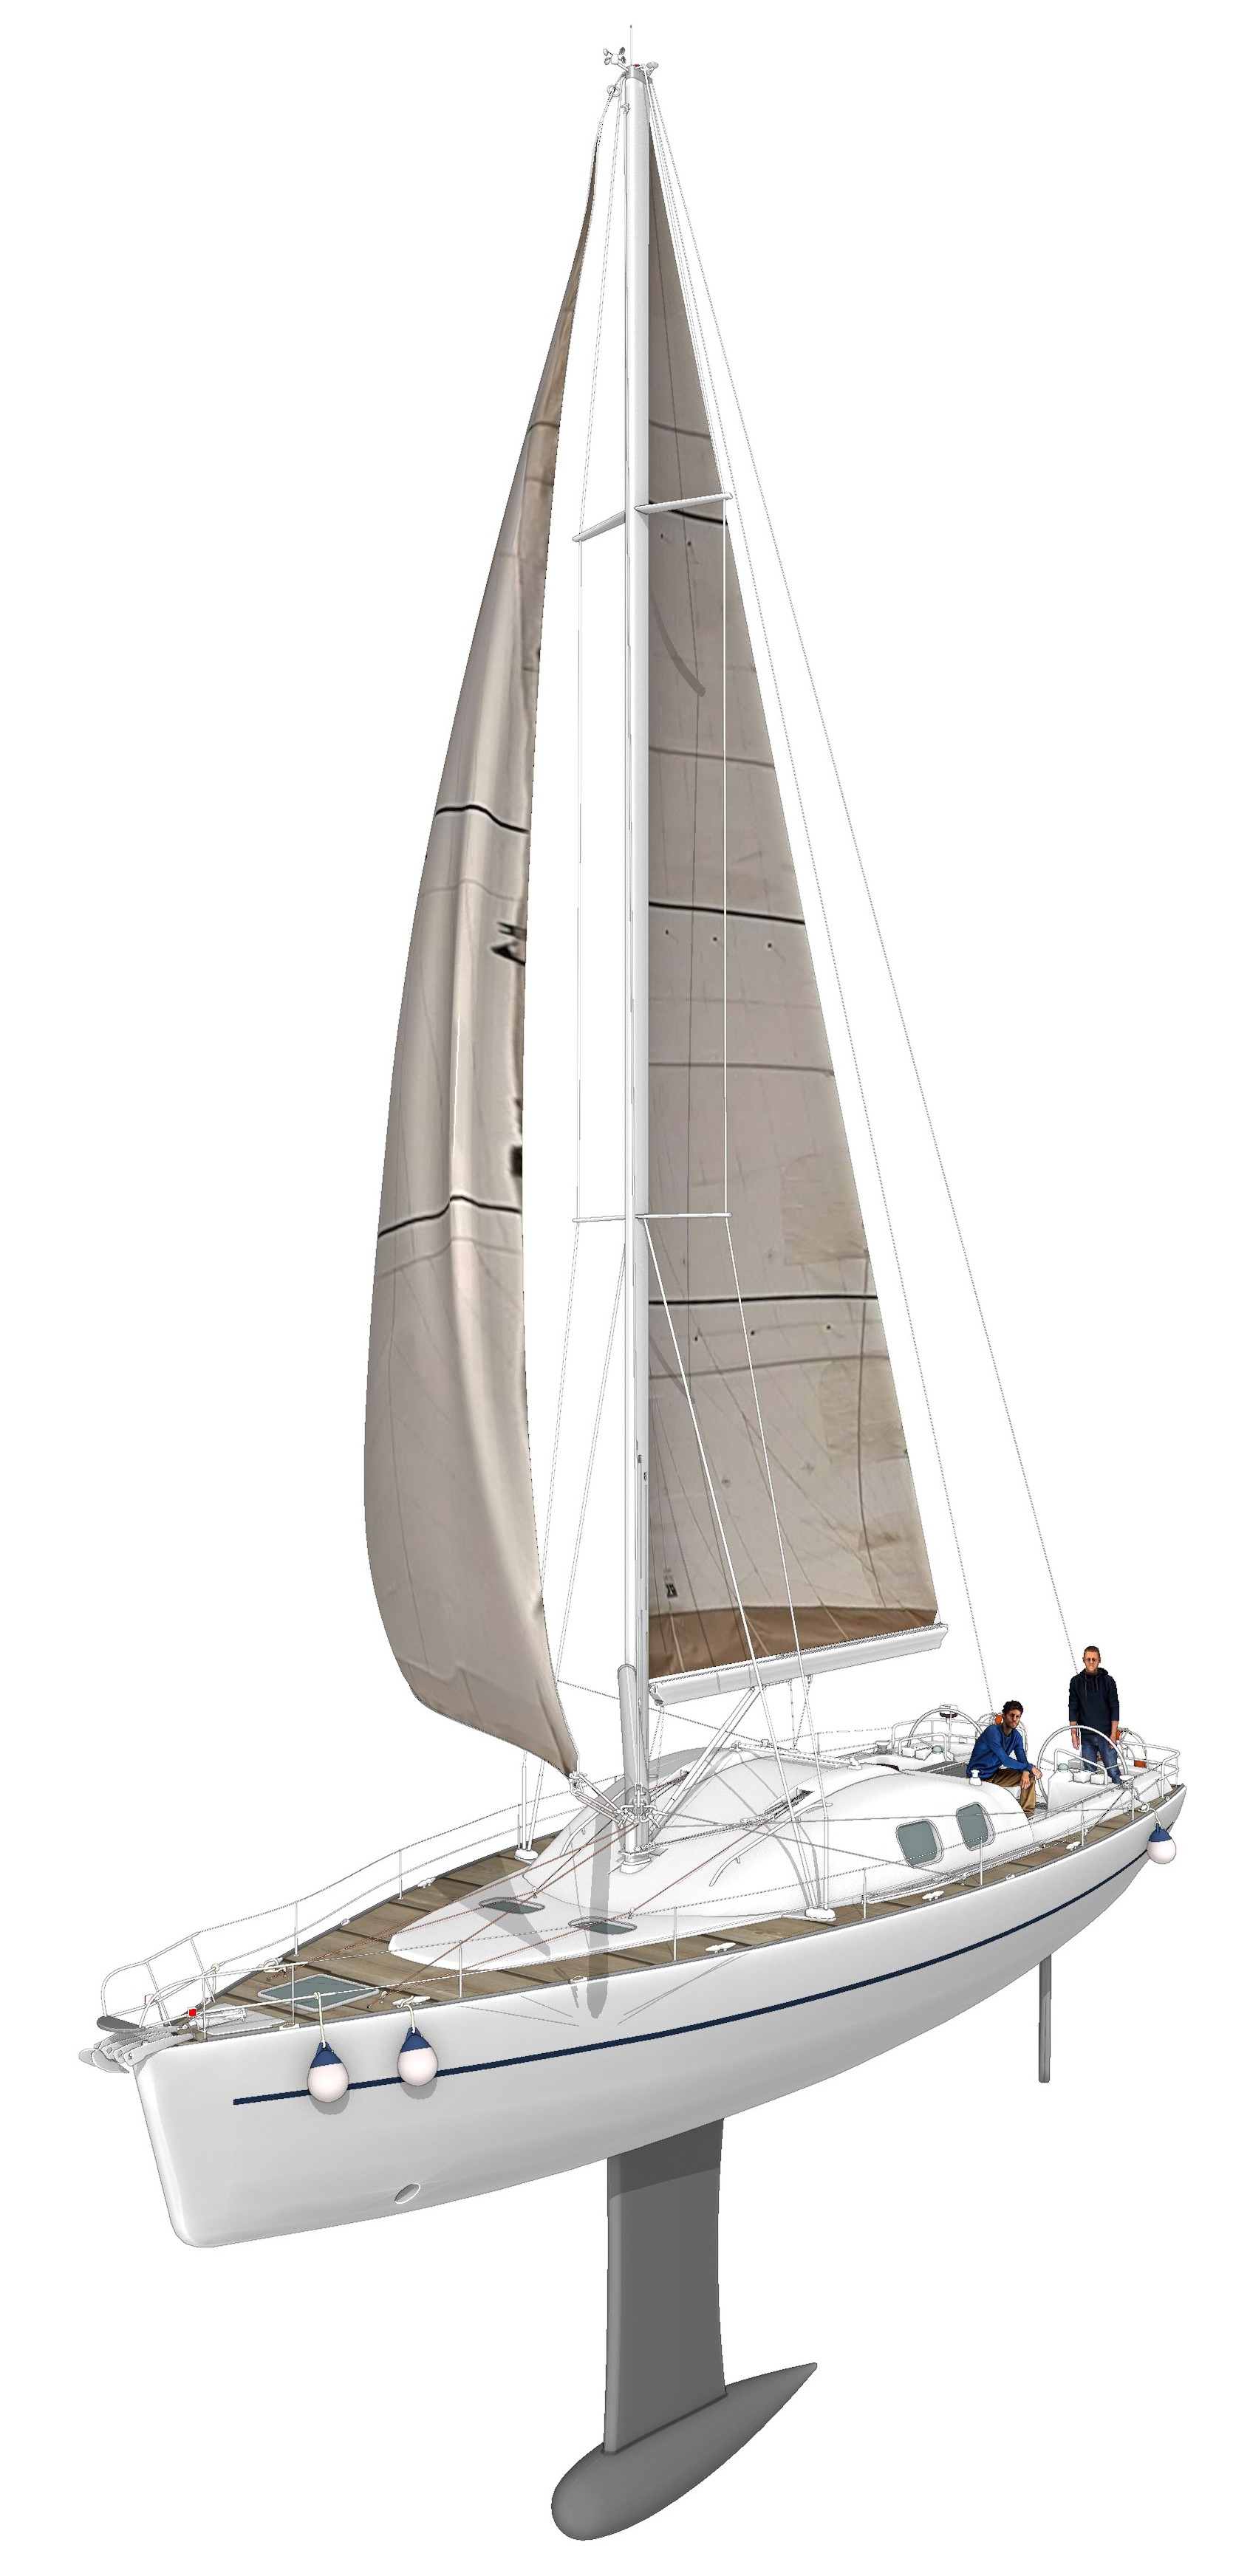
\includegraphics[width=\textwidth]{gfx/prod/boat/boat.jpg}


\section{Erstellung der Drohne}

\subsection{Photoscan und CAD Daten}

ca 250 fotos mit iphone
perspektive so, dass alles abgedeckt ist
trotzdem haben seiten gefehlt
(bild von scan)
weitere cad daten wurden von cadgrab heruntergeladen
es muss ja nichts modelliert werden, was schon vorhanden ist.
dazu gehören der elektromotor, servomotoren, propeller.

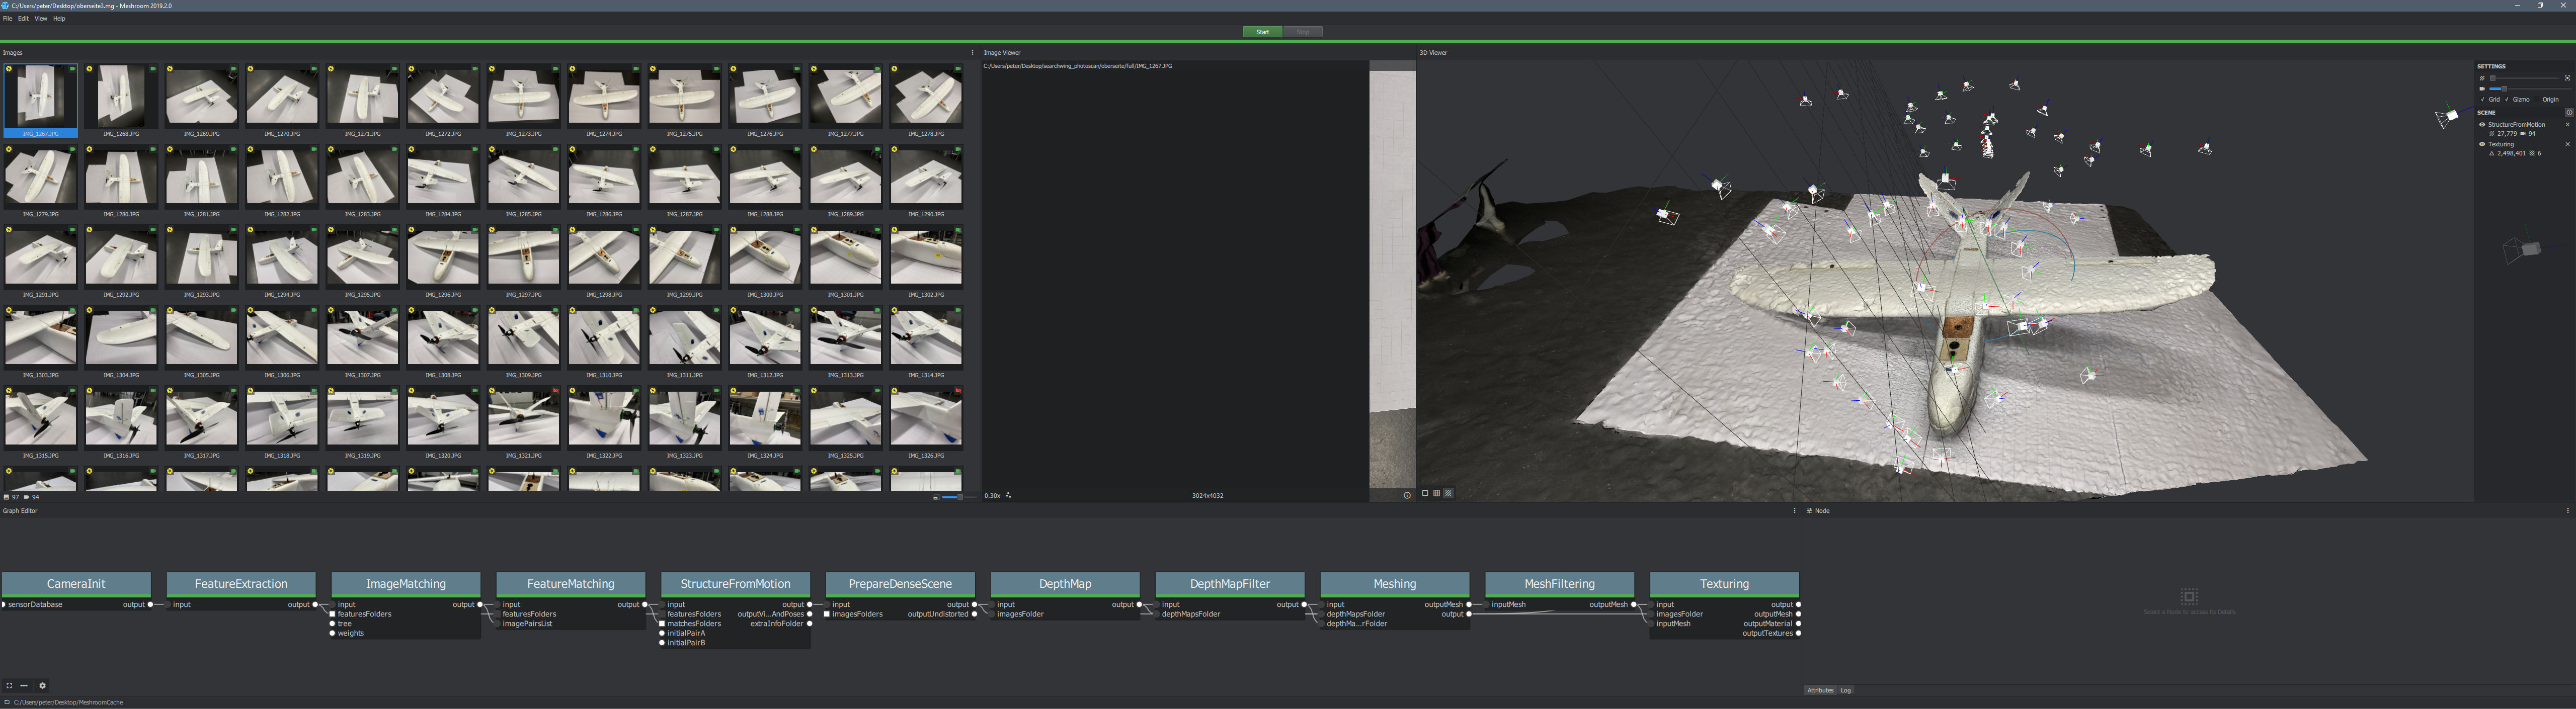
\includegraphics[width=\textwidth]{gfx/prod/plane/meshroom1.jpg}
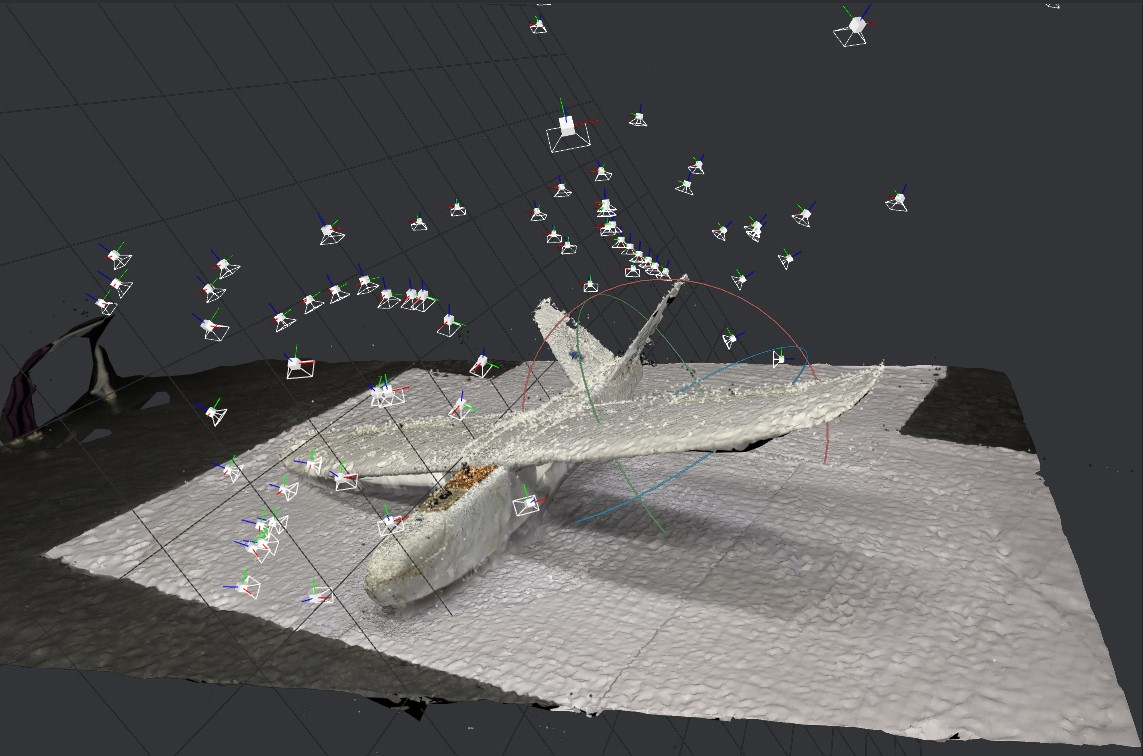
\includegraphics[width=\textwidth]{gfx/prod/plane/meshroom2.jpg}


\subsection{Modellierung}

das importierte cad und photoscan wurde teilweise komplett neumodelliert (flügel, Leitwerke, )
Kleinteile wurden ebenfalls selbstmodelliert.
der Rest waren CAD-Daten wie oben beschrieben

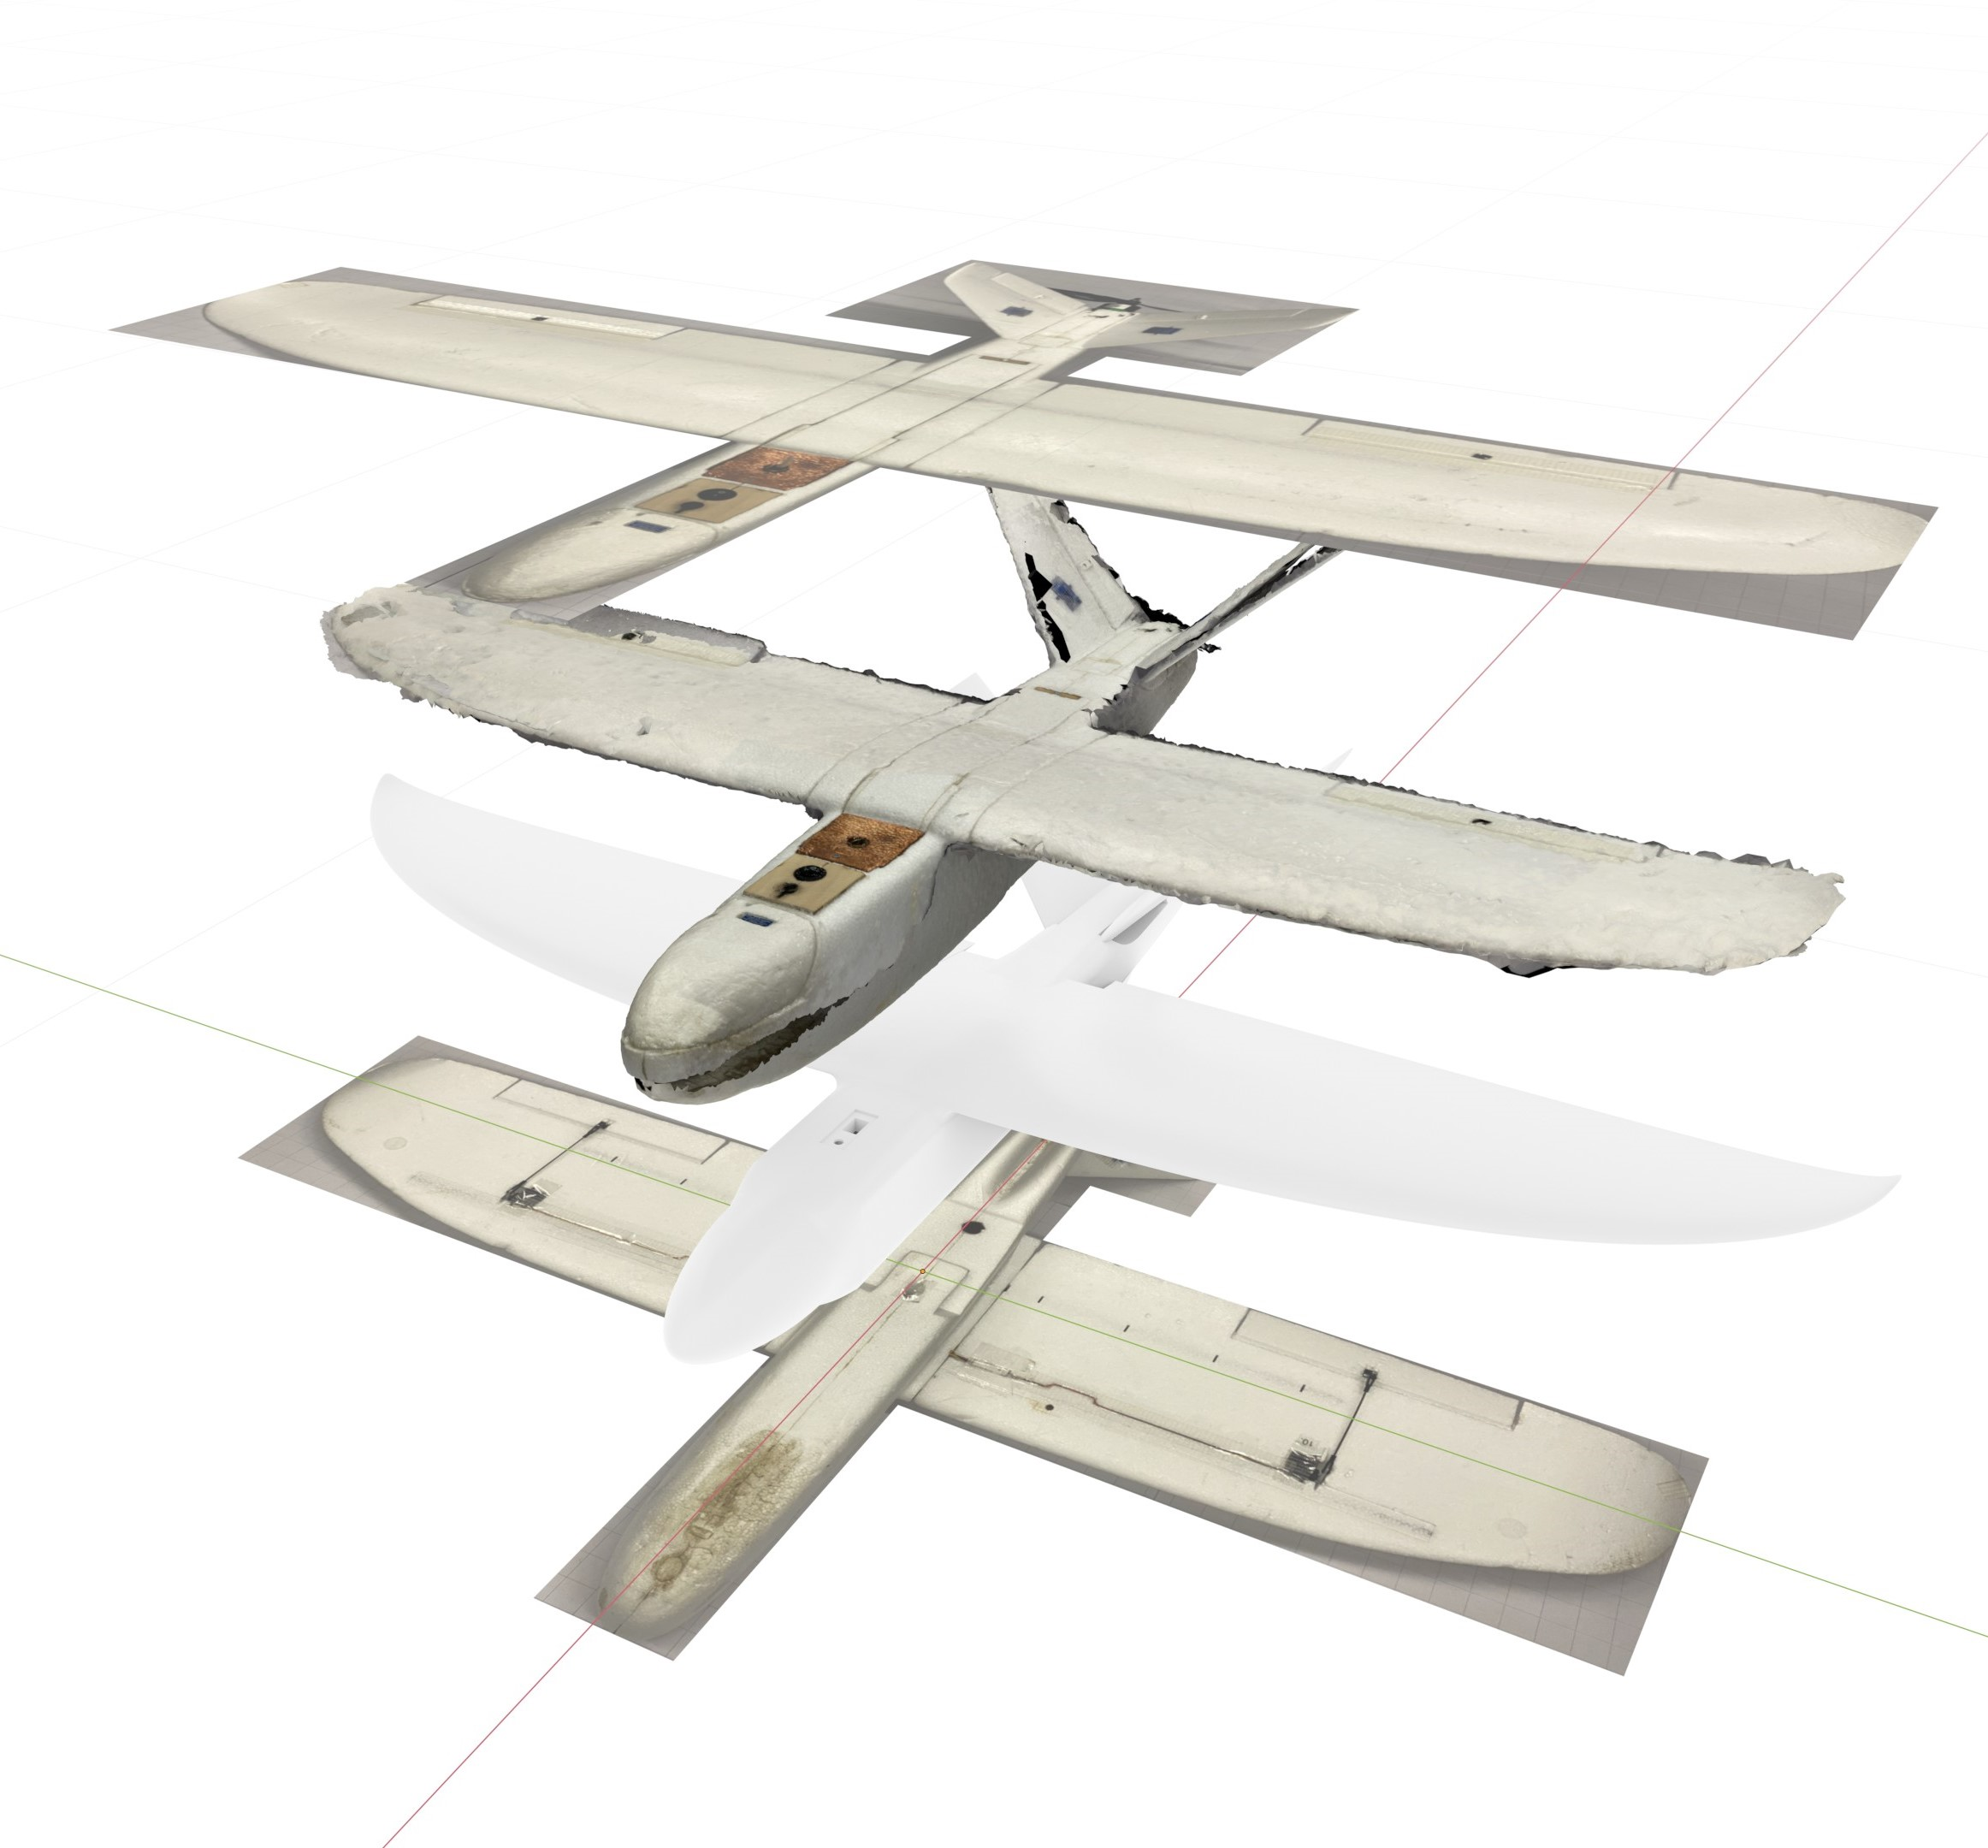
\includegraphics[width=\textwidth]{gfx/prod/plane/plane5.jpg}
\subsection{shading + look}

prozedurale voronoi textur als basis für das Styropor. 
dies war wichtig, da eine vernünftige uv-layer nicht angelegt werden konnte, da die topologie an dem cad-import sich hierfür schlecht geeignet hat
mit glossy shader und subsurface scattering konnte der nötige Realismus erreicht werden.
die restlichen objekte waren ganz gewöhnlich geshadet

hinweis auf intro text
unterschiedliche textgrößen, damit klar ist, dass titel untertitel und keine information
weißter text mit milchglassähnlichem rahmen damit zu restlichen film durchgängiger look ist


\includegraphics[width=\textwidth]{gfx/prod/env/intro_text.jpg}


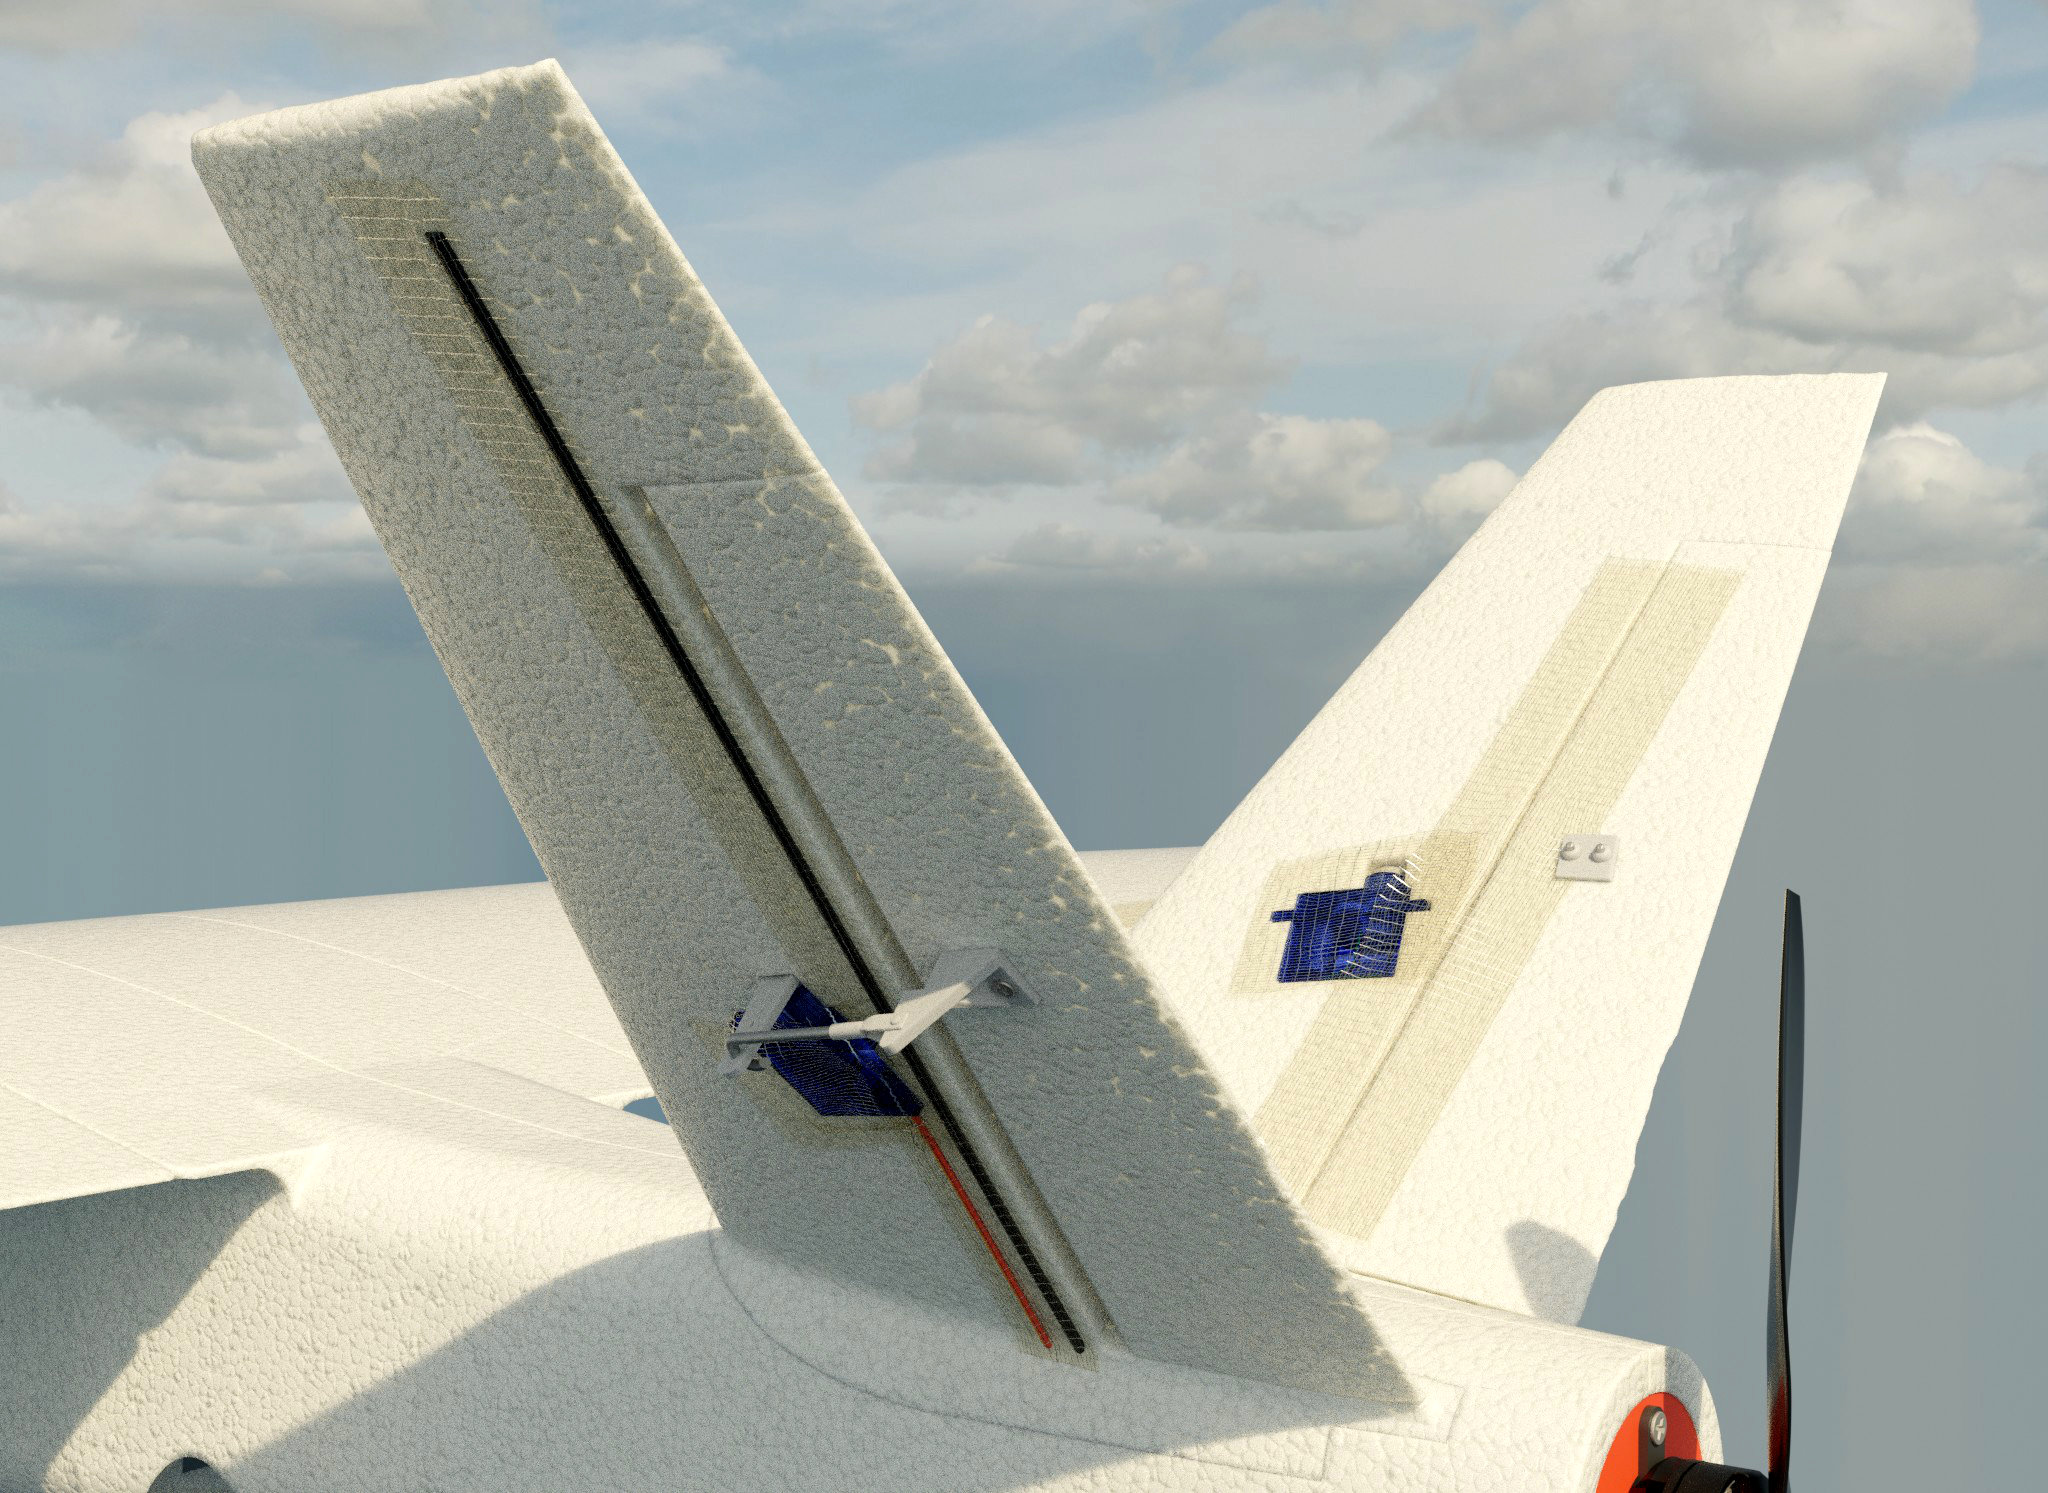
\includegraphics[width=\textwidth]{gfx/prod/plane/shading.jpg}


was den look angeht, wurde ein möglichst realistischer angestrebt, damit sich die gerenderten szenen sich möglichst gut in den film integrieren und der zuschauer nicht von unterschiedlichen looks verwirrt ist

\subsection{Rigging und Animation}

Die Gelenke der Servomotoren wurden mit einem inverse-kinematik rig versehen. Somit haben sich die Stangen und auch der Hebel an dem Servomotor mitbewegt.
am ende waren die bewegungen der Servomotoren nur abhängig von einem einzigen bone, der wie ein steuerruder bei einem flugzeug funktioniert hat.
wurde der Steuerknüpel nach vorne geneigt, haben sich bspw. die hinteren beiden  leitwerk nach unten bewegt
die klebebänder müssen sich entsprechend deformieren.
daher hier weightpainting


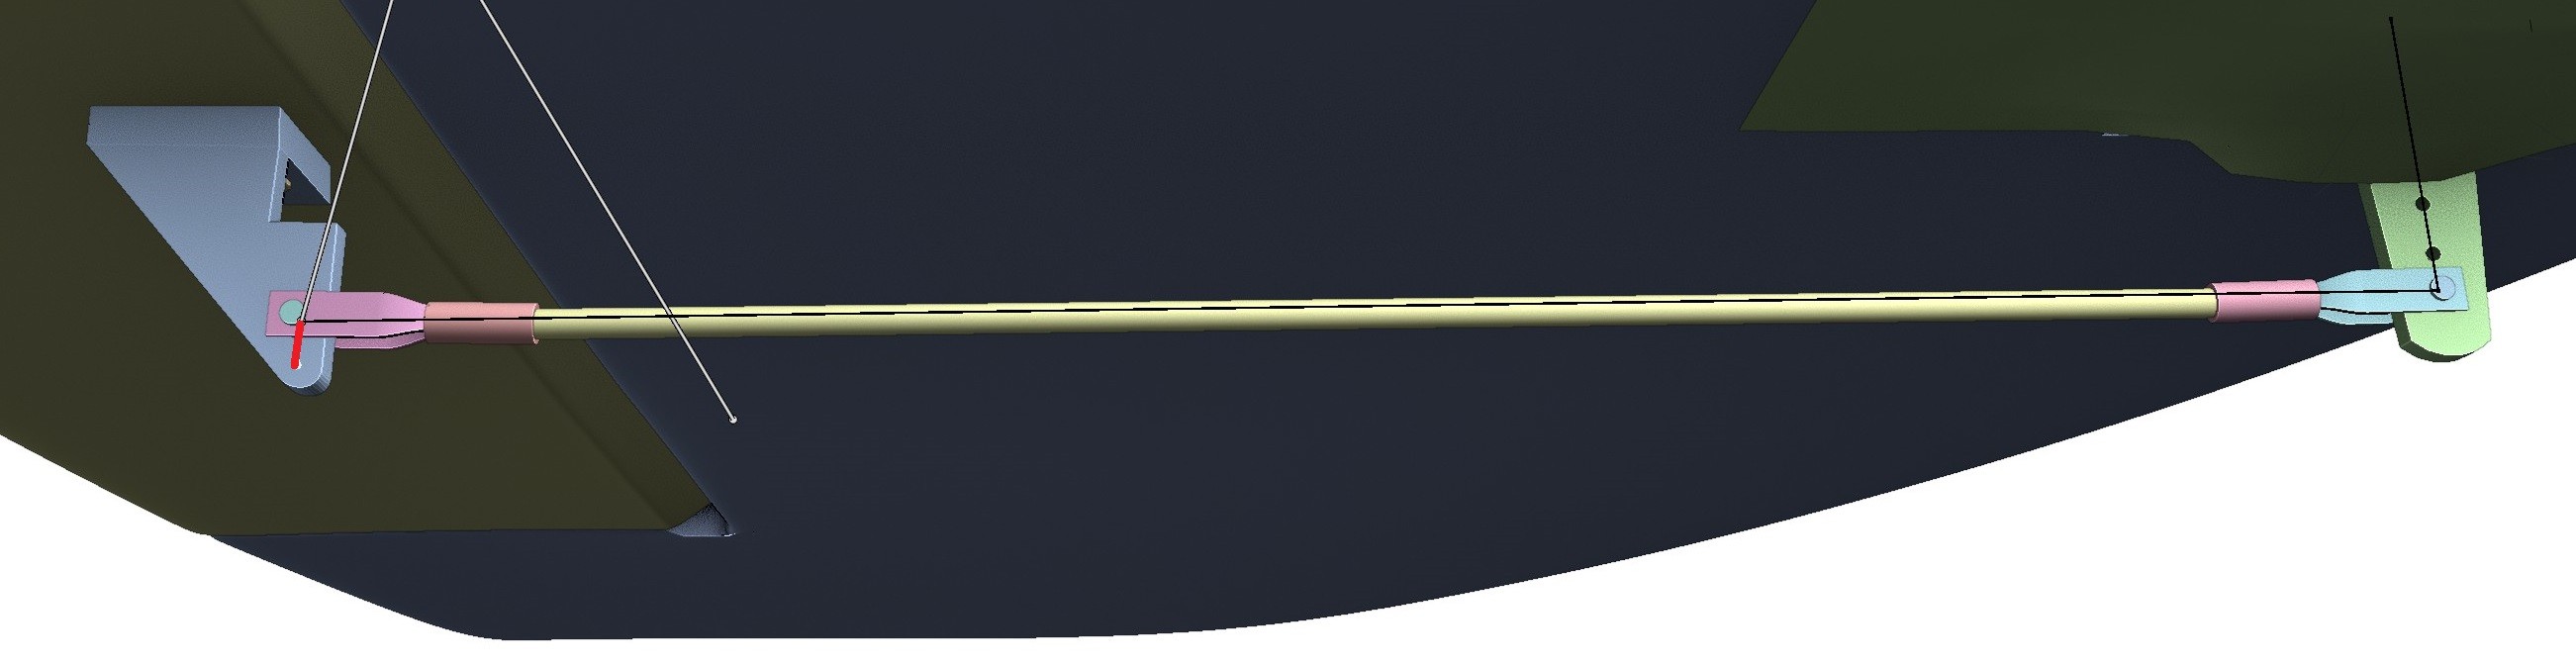
\includegraphics[width=\textwidth]{gfx/prod/plane/plane7.jpg}
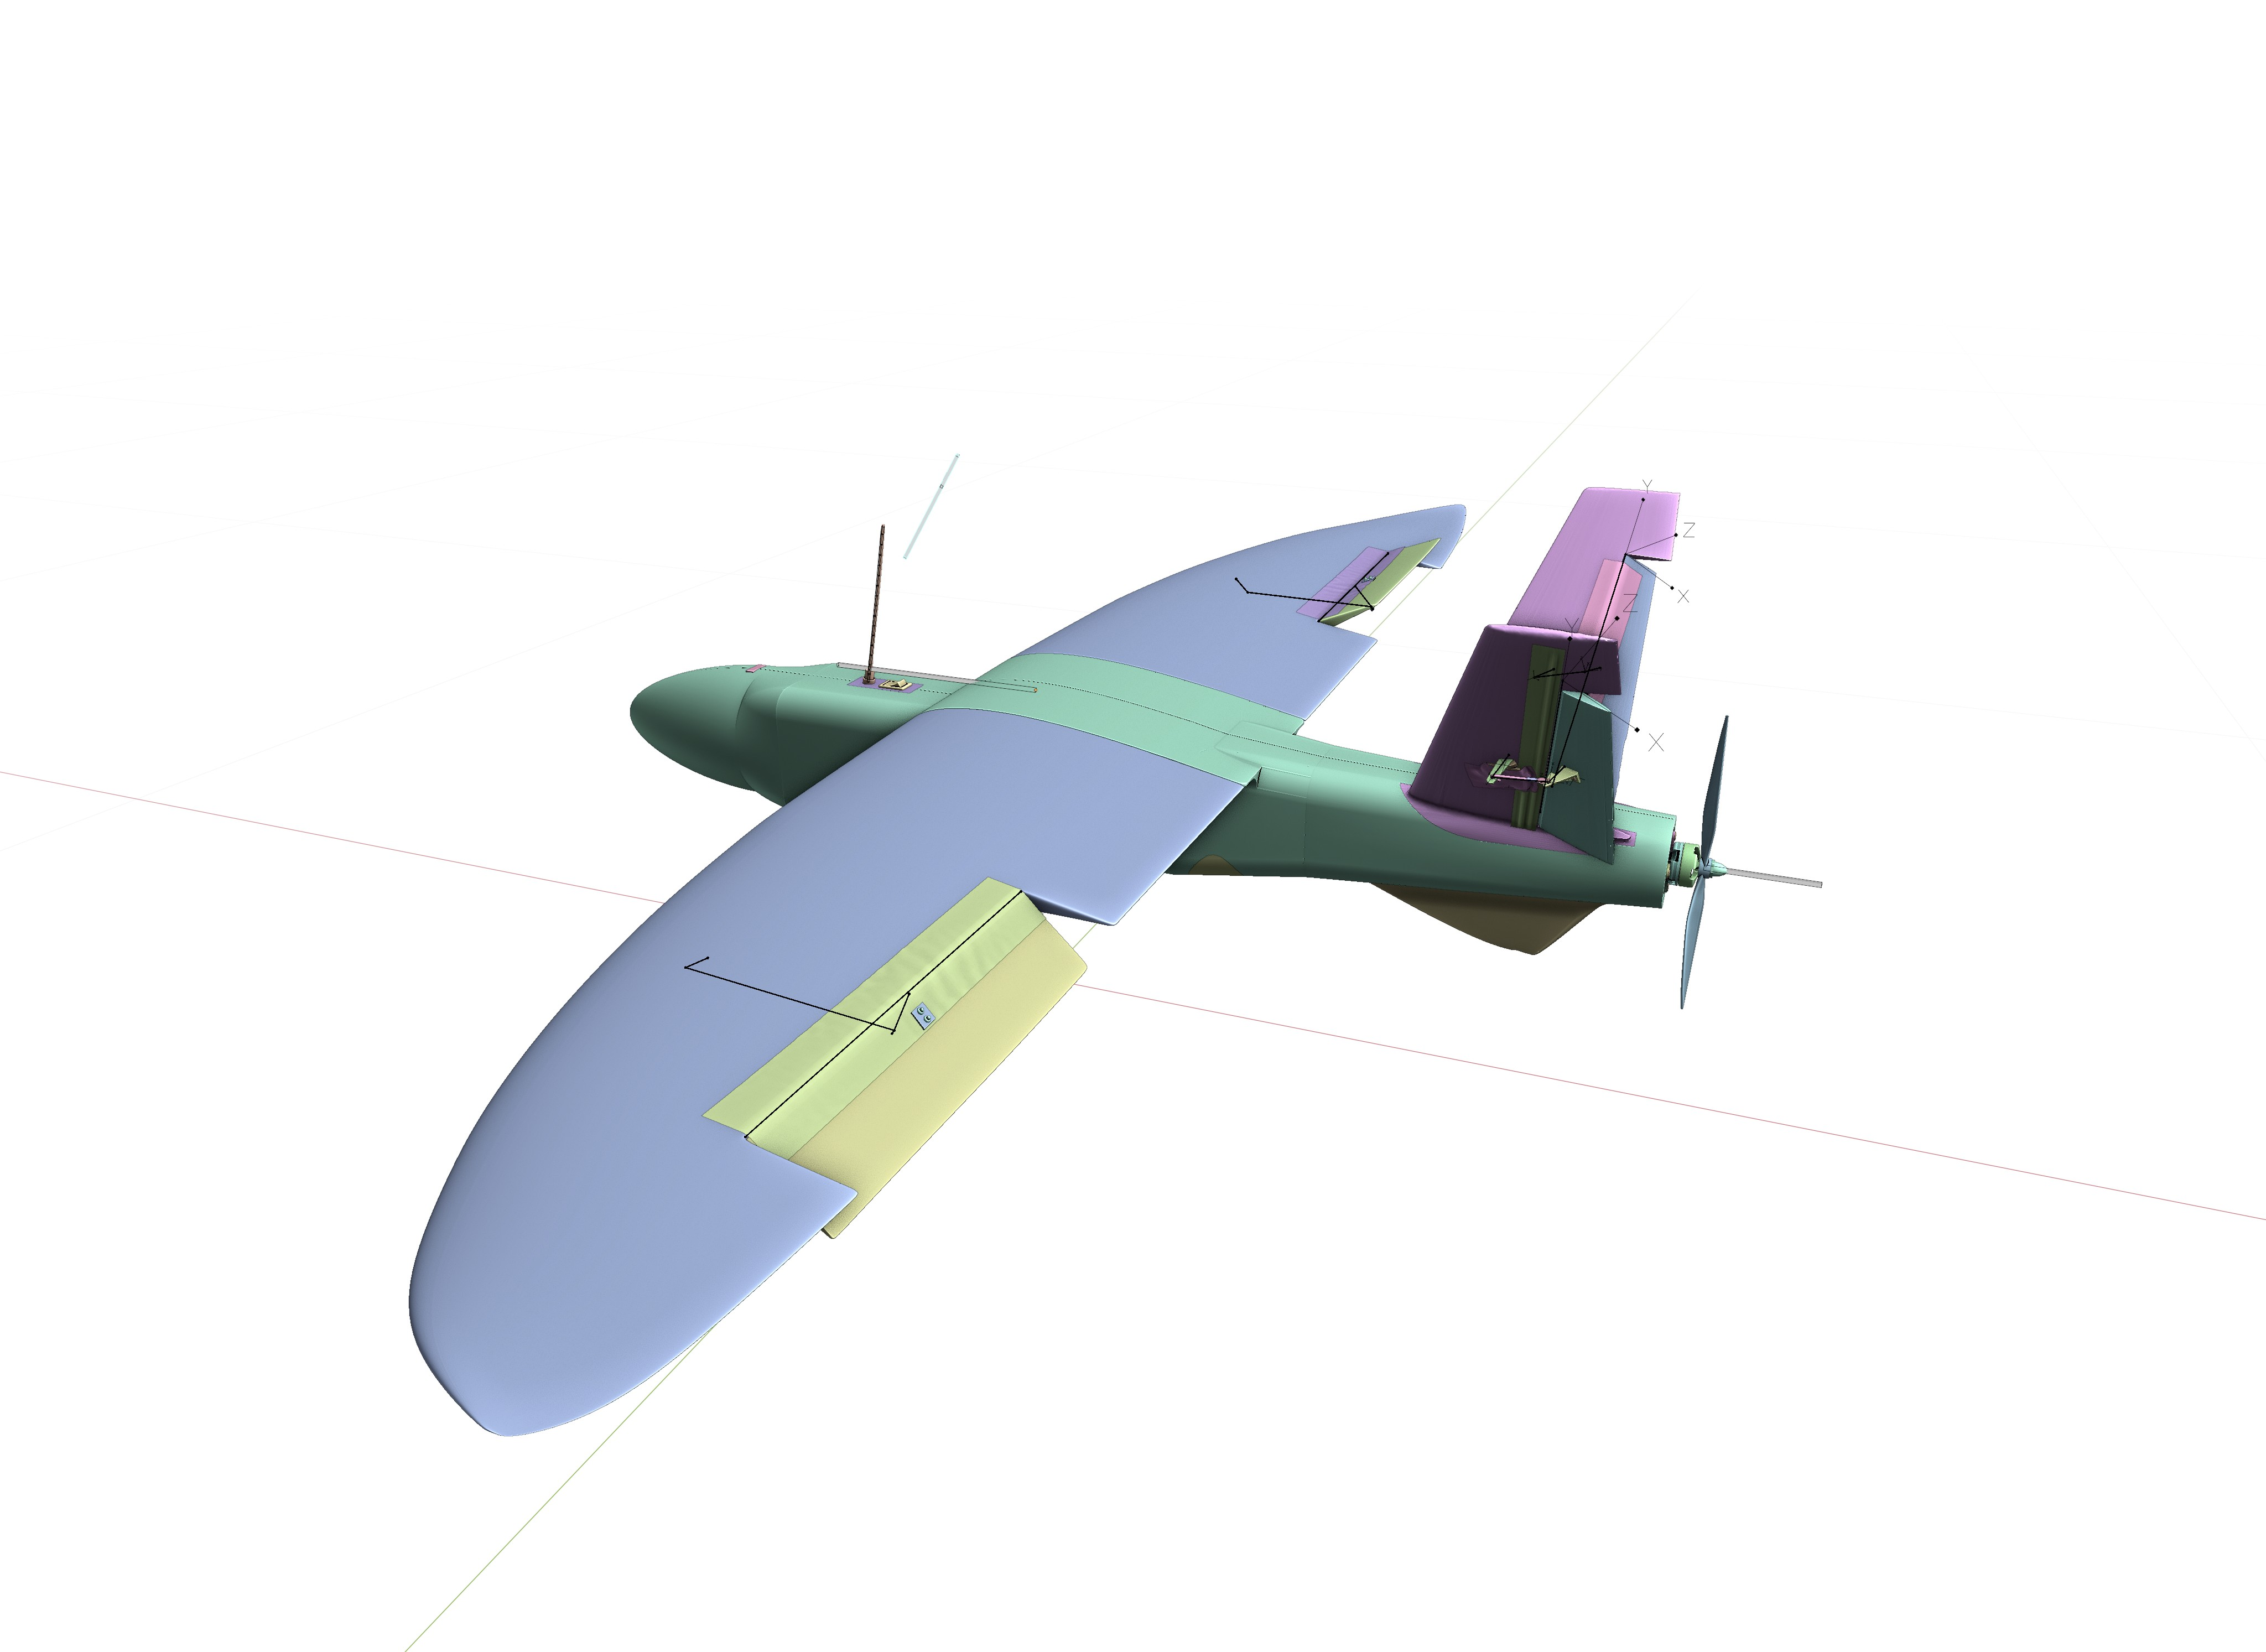
\includegraphics[width=\textwidth]{gfx/prod/plane/plane8.jpg}

\section{Animation}

animation nodes setup: Flugzeug bewegt sich der gegebenen kurve entlang und stellt neigung und die Klappenstellung automatisch ein
kamera wurde klassisch gekeyframet
besonderheit hierbei war, dass ein child-of constraint in die kamera eingefügt wurde, welches von der position des flugzeuges abhängig ist.
so bewegt sich die position der kamera mit dem flugzeug mit, aber es dreht sich nicht mit. zusärtlich zu diesem constraint wurden keyframes eingefügt, sodass die kamera sich praktisch relativ zum flugzeug bewegt.
dies war eine sehr große erleichterung bei der erstellung der animation
auch weil wenn sich die position des flugzeuges durch bspw. anpassen des pfades, die kamera immernoch beim flugzeug geblieben ist.
manuelle keyframe animation für landung + kamera

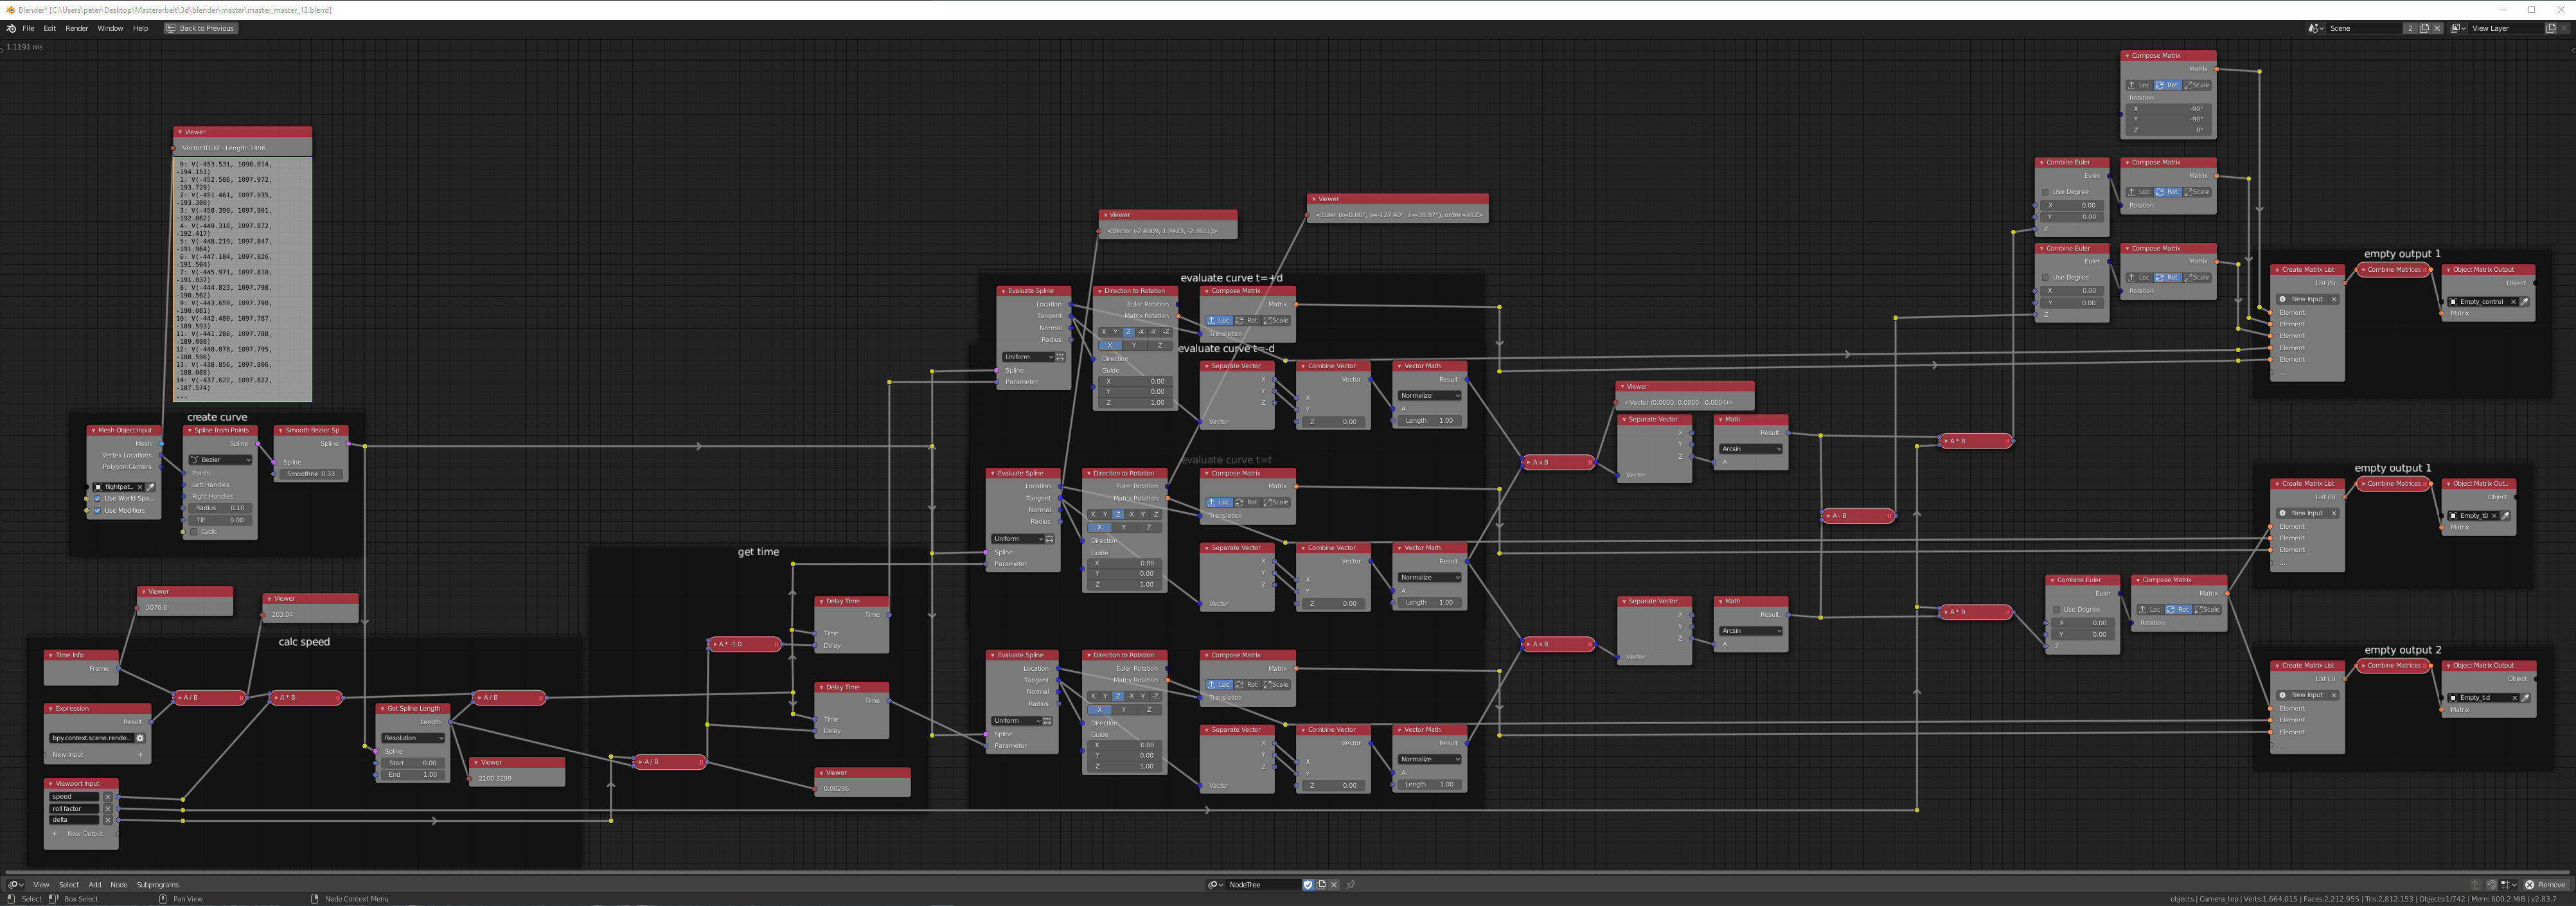
\includegraphics[width=\textwidth]{gfx/prod/plane/animation_nodes.jpg}
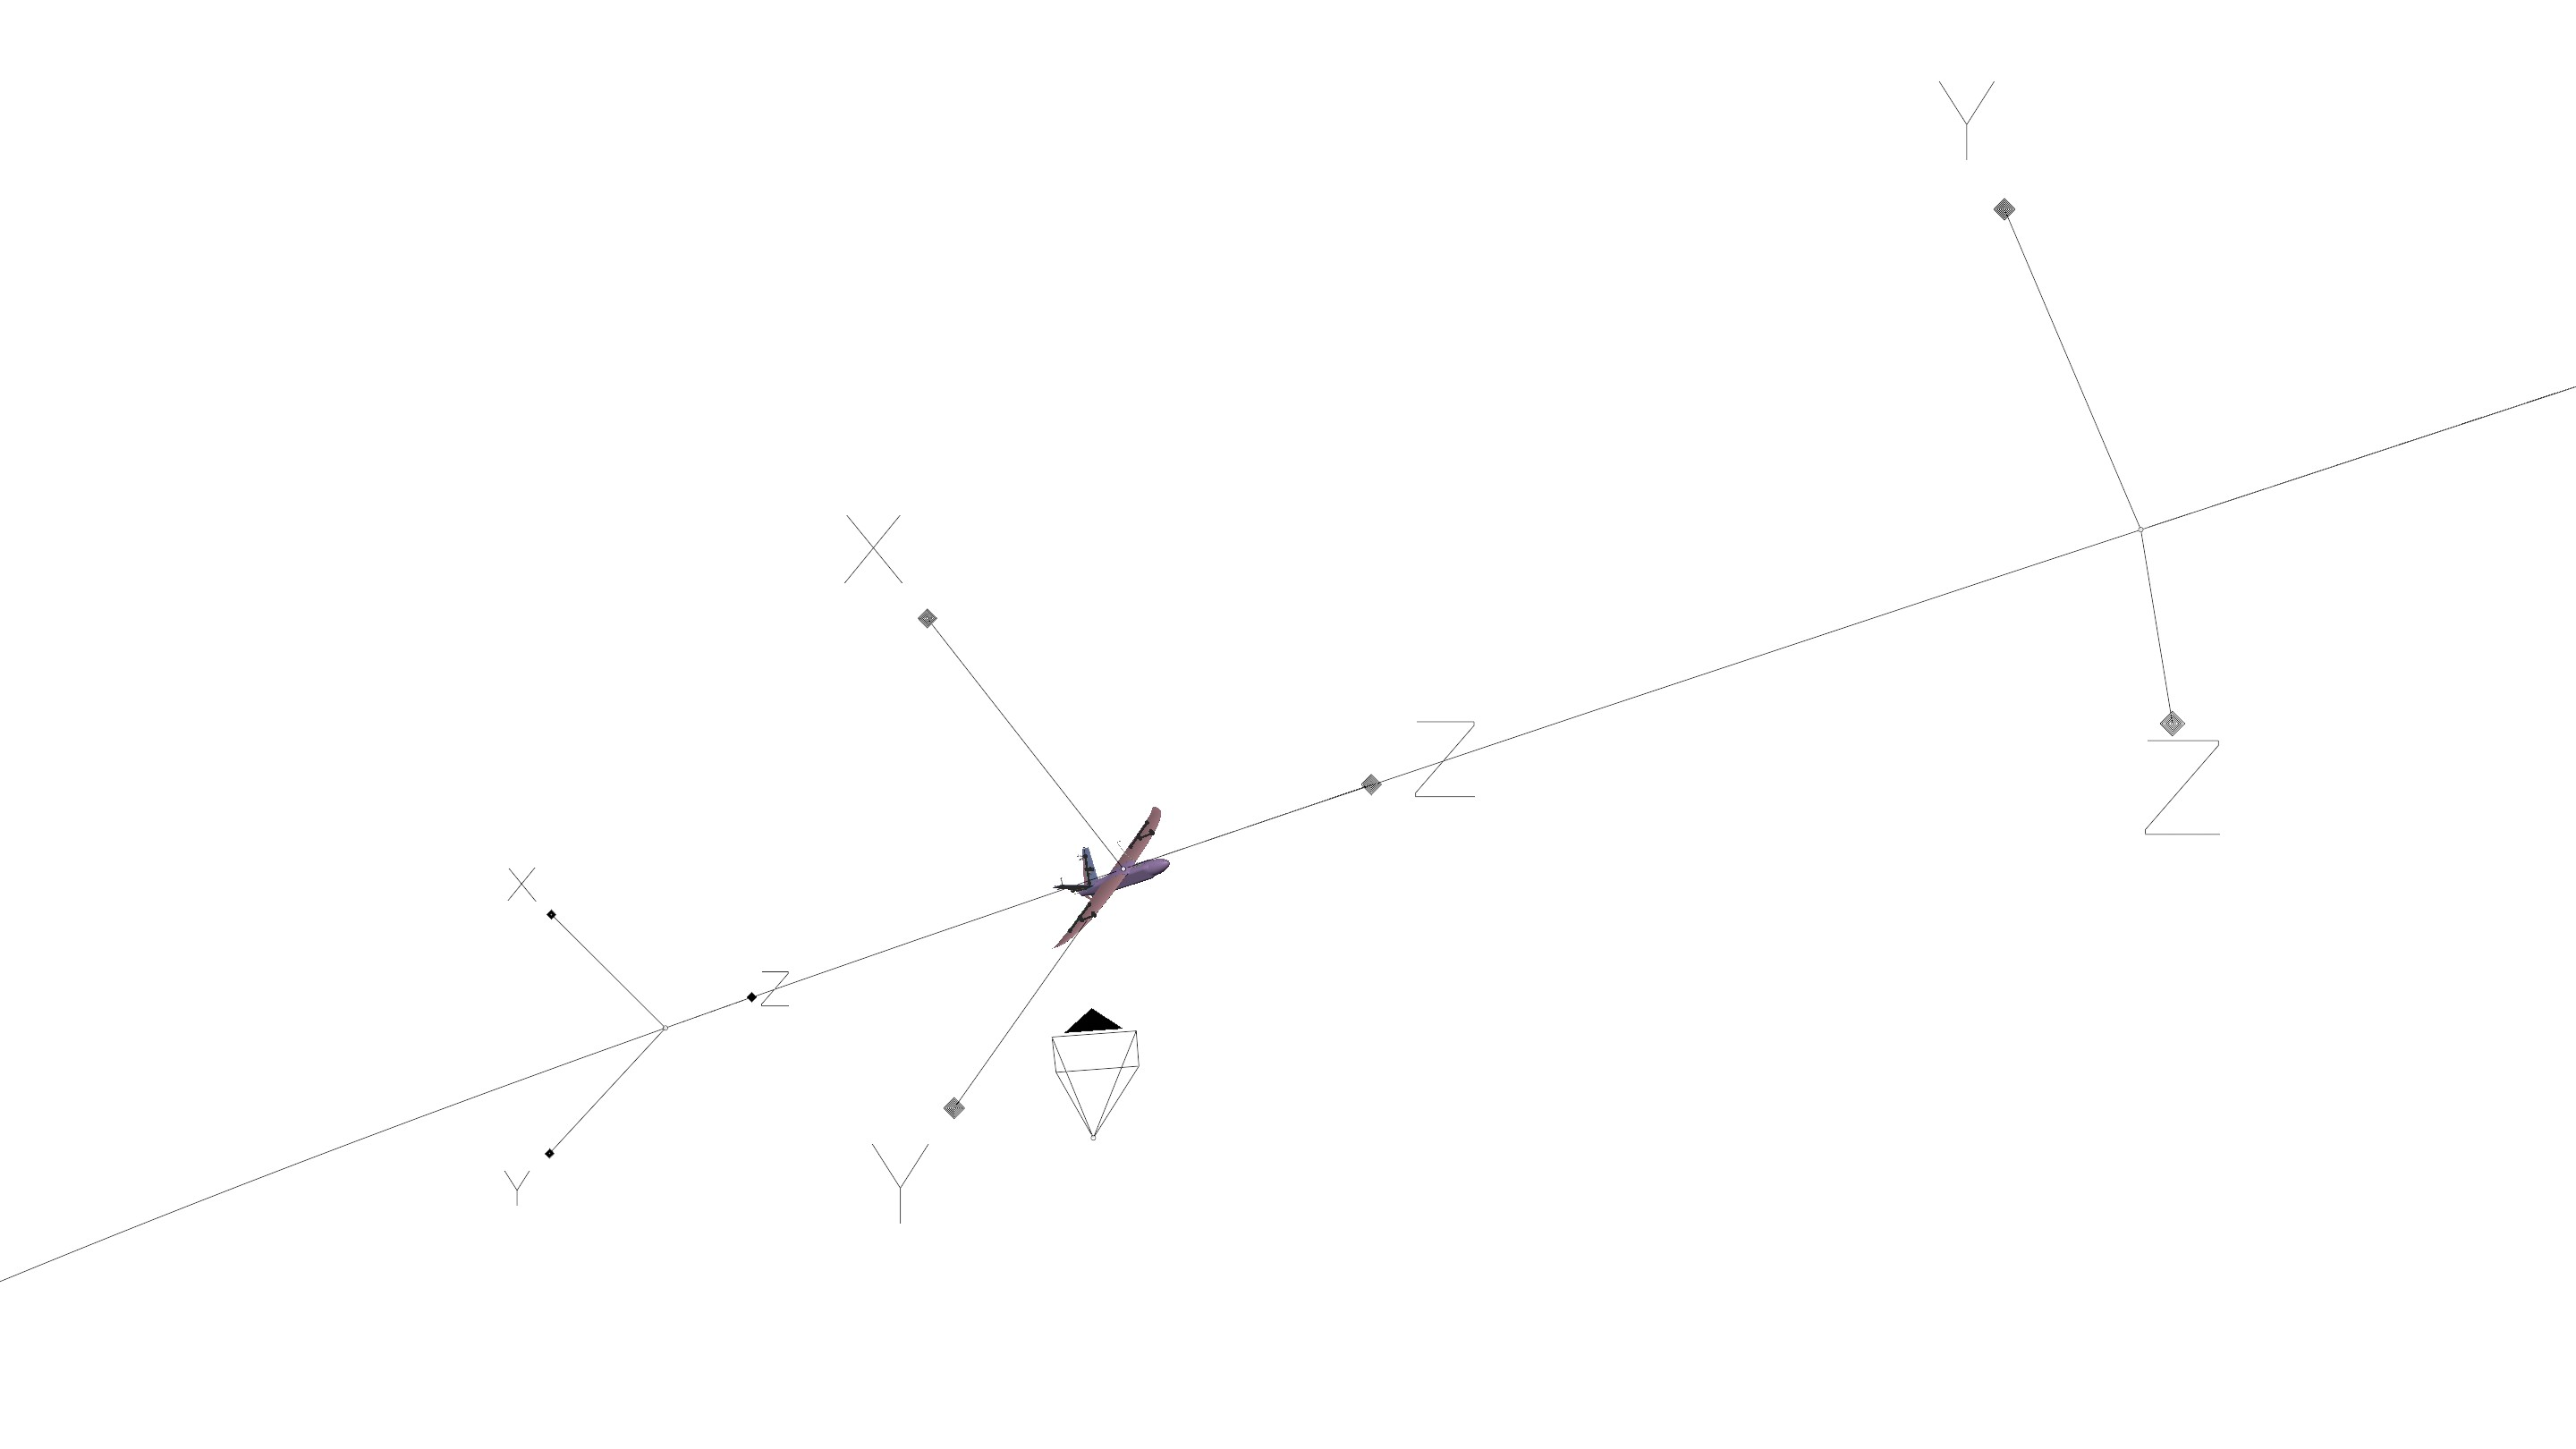
\includegraphics[width=\textwidth]{gfx/prod/plane/an_flight.jpg}

\section{Spezialeffekte}

partikelsystem für landung

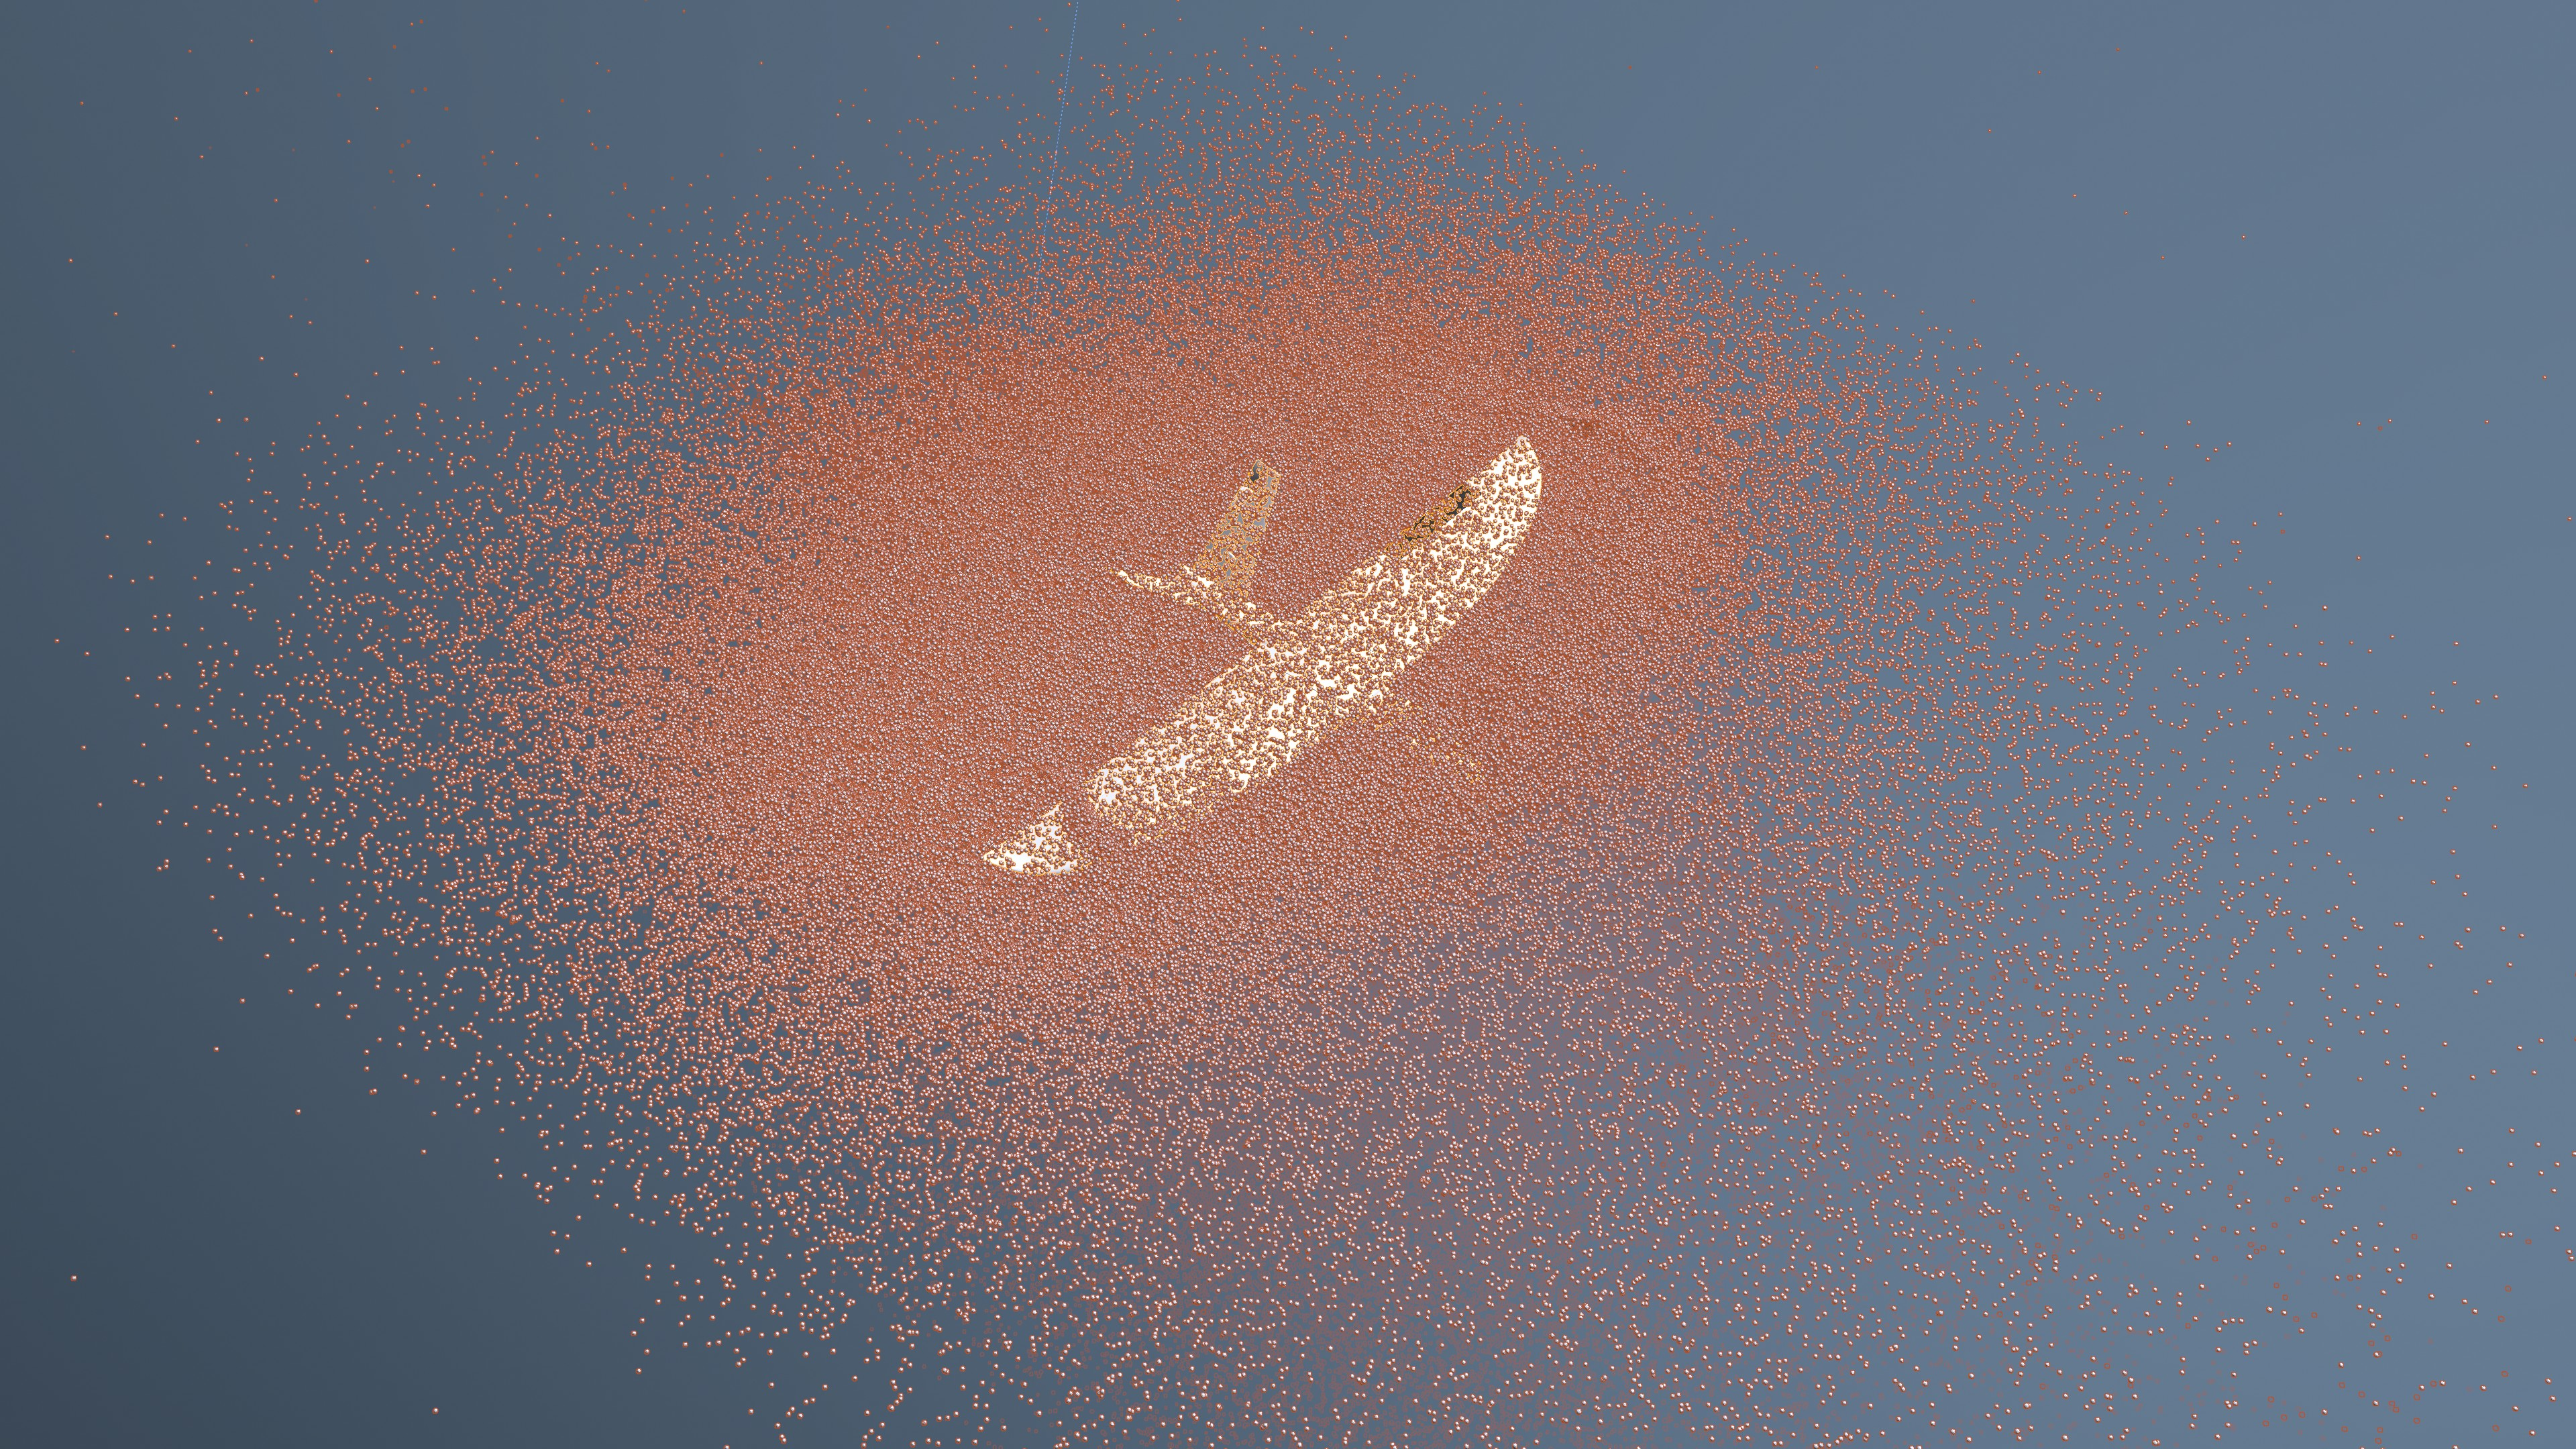
\includegraphics[width=\textwidth]{gfx/prod/plane/particles.jpg}

\section{Rendering und Datenhandling}

rendering in der cycles engine
da ein schönes visuelles ergebnis hier leichter zu erreichen ist wie in eevee
mehr realismus --> wichtig, da 3d in realfilm integriert wird
denoising wurde über export von multilayer openexr möglich gemacht
also nach dem rendering wurden die bildern denoist

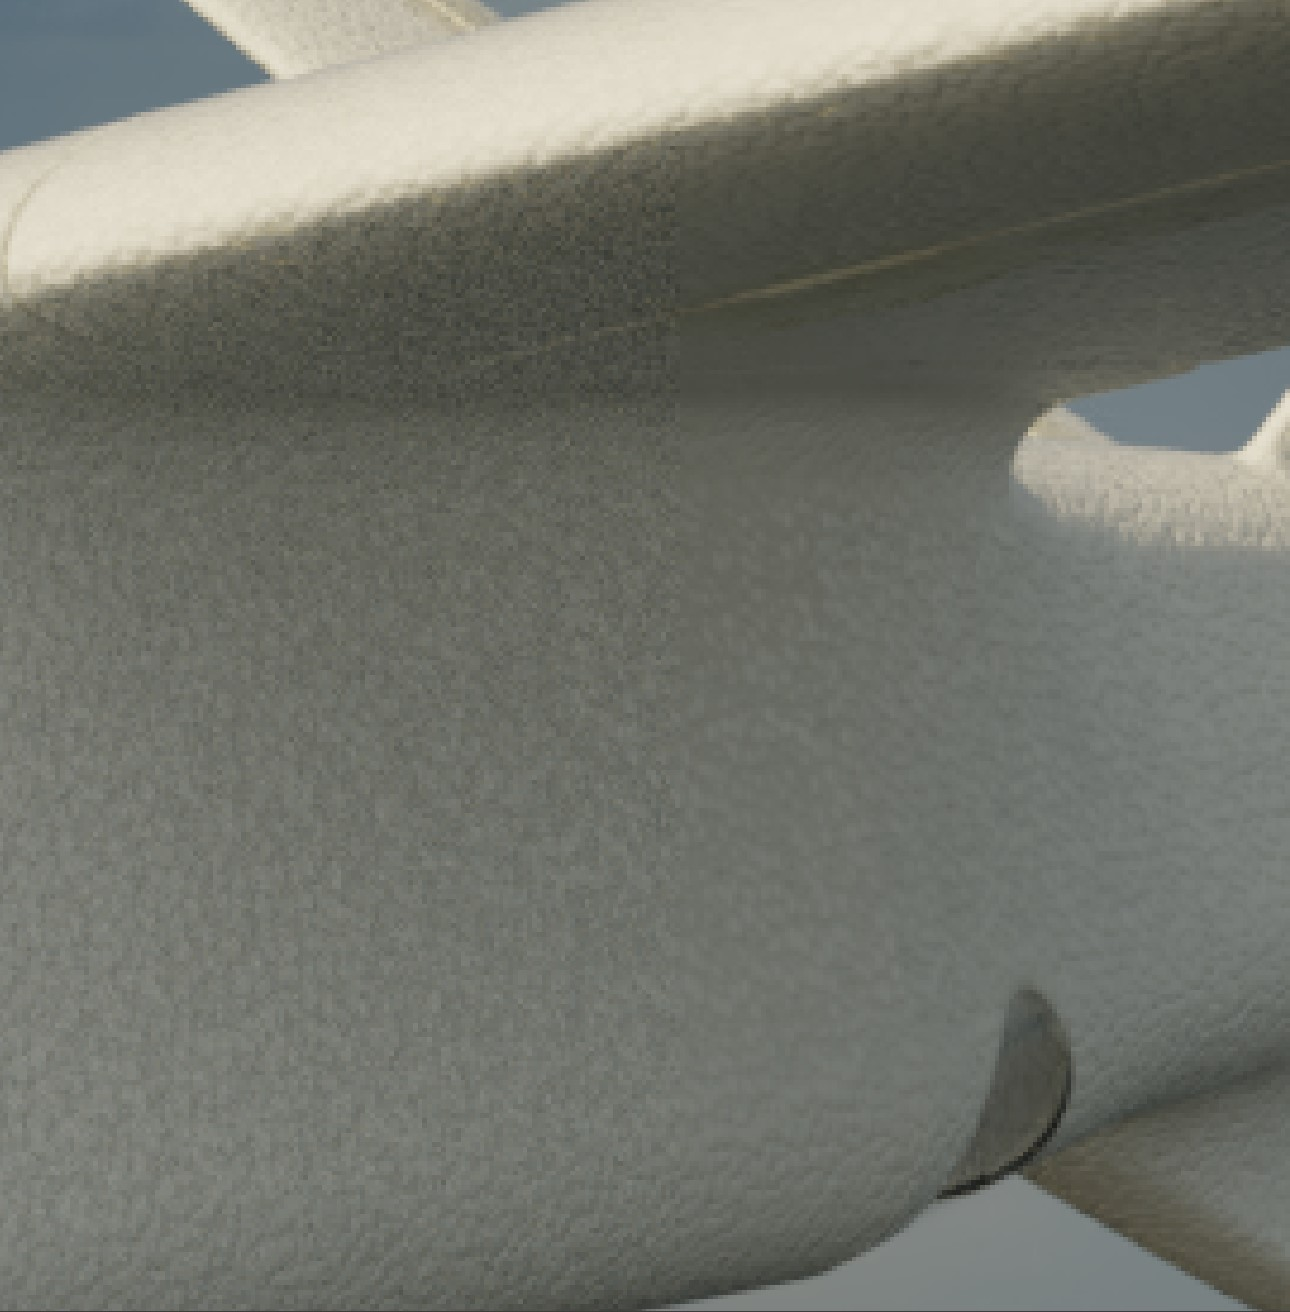
\includegraphics[width=\textwidth]{gfx/post/denoising.jpg}
einziger nachteil dieses workflows sind die sehr großen datenmengen. somit hatten alle gerenderten bilder mit versionen eine datenmenge von etwa 1,2 TB
in den insgesamt 5 szenen (intro, flug erster teil, flug zweiter teil, landung und outro) etwa 1550 Bilder.
mit einer renderzeit von etwa 1,5 minuten pro bild, belief sich die renderzeit pro iteration auf knapp 40 Stunden.

probleme von genauigkeiten beim rendern
weil single float precision
umso näher am urpsorung umso besser
daher wurden die szenen mit keyframes nach bedarf verschoben

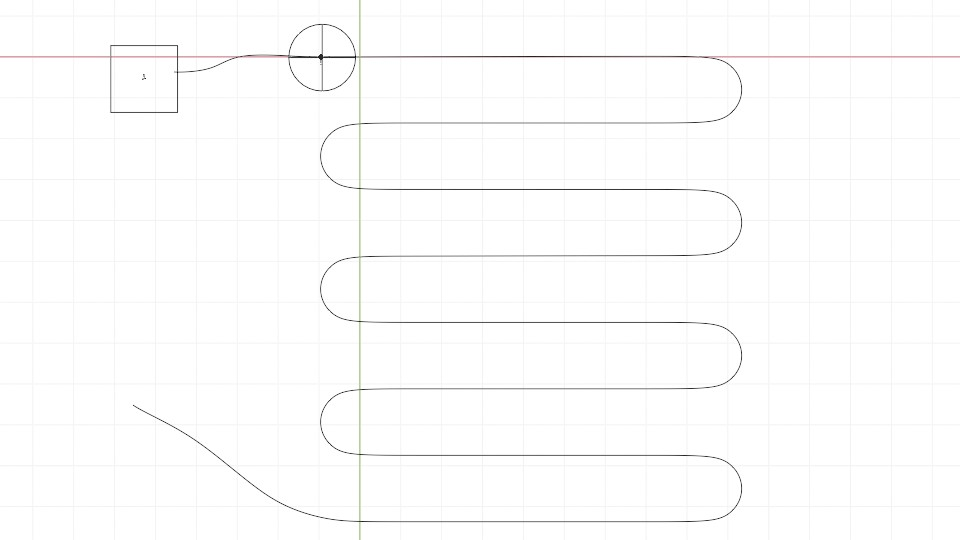
\includegraphics[width=\textwidth]{gfx/prod/plane/flightpath1.jpg}
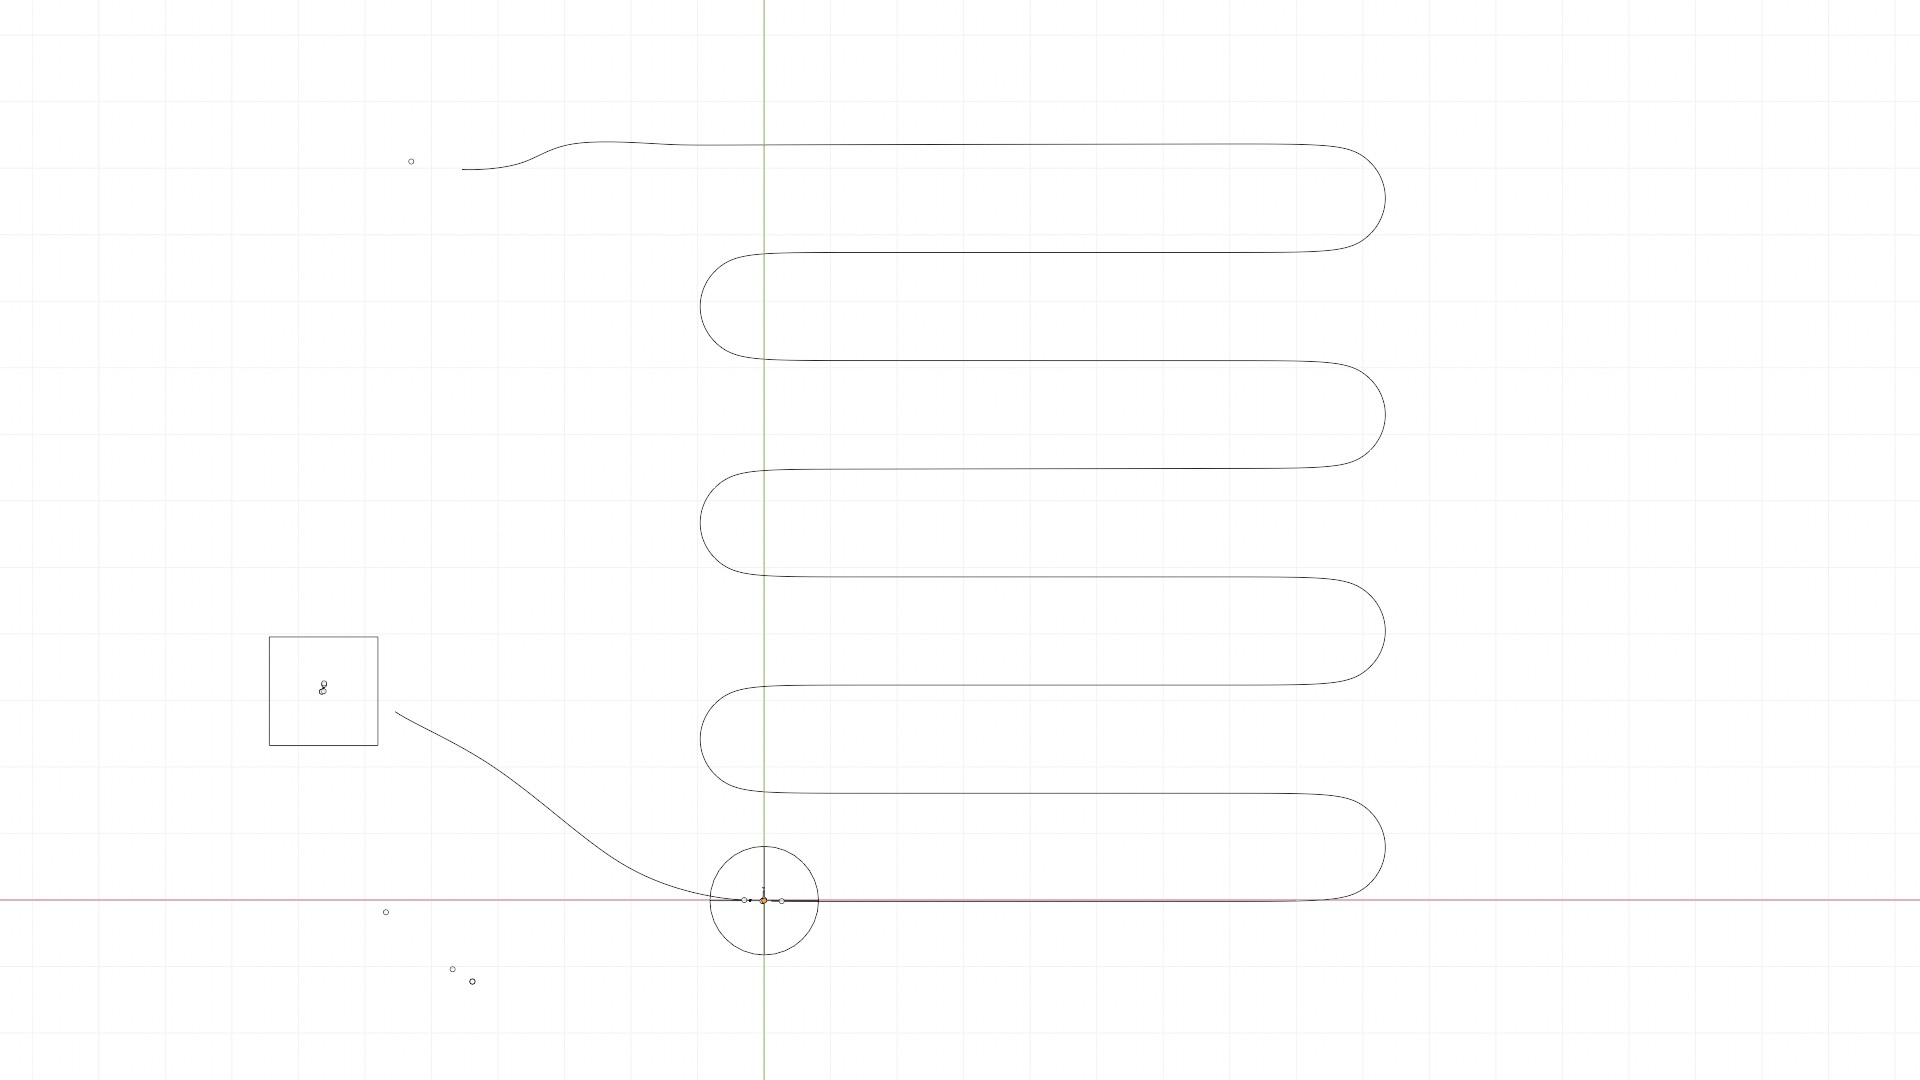
\includegraphics[width=\textwidth]{gfx/prod/plane/flightpath2.jpg}



% Bilder von denoising?
